% TRUTH VERSION: elite_status-v04.tex
% FILE ROLE: AUTHORITATIVE MANUSCRIPT
% PREVIOUS TRUTH VERSION: elite_status-v03.tex; SUPERSEDED
% BASE SHA256 (elite_status-v03.tex): 721eab3beee8956680f68d3851637e434d231de53a45a1c31a24c12977ab0762
% PRE-PROMOTION POSITIONING CANDIDATE SHA256: 8cf7c6280262b038677417553ae1906416c8a672ec867cb4f9a9337c863f5398
% EARLIER TRUTH VERSION: elite_status-v02.tex; SUPERSEDED
% V03 PRE-PROMOTION CANDIDATE SHA256: 2c5be85a58fb60ad6152424fe0ebdb35081b0246951ef27829489de6953eccf7
% BASE SHA256 (elite_status-v02.tex): 1a25382edf830d9008ec7bd6b667f124c0a95783a0cf424fd5763ebcbdc31c5c
% PORTABILITY SUBBRANCH SHA256: d77fad7748d2a287ad9ff3657beaaf7d947f8511695d825befc6dae693ee8245
% DOCUMENT: Journal of Political Economy Draft


\documentclass[12pt,letterpaper]{article}
\usepackage[utf8]{inputenc}
\usepackage{amsmath,amssymb,amsthm}
\usepackage{graphicx}
\usepackage{natbib}
\usepackage{booktabs}
\usepackage{setspace}
\usepackage{geometry}
\usepackage[colorlinks=true,citecolor=blue,linkcolor=blue]{hyperref}
\geometry{margin=1.1in}

\newtheorem{theorem}{Theorem}
\newtheorem{proposition}{Proposition}
\newtheorem{lemma}{Lemma}
\newtheorem{corollary}{Corollary}
\newtheorem{assumption}{Assumption}
\newtheorem{remark}{Remark}
\theoremstyle{definition}
\newtheorem{definition}{Definition}

\newcommand{\Lists}{\Lambda}
\newcommand{\R}{\mathbb{R}}

\title{The Market for Elite Status\thanks{Working draft --- not for circulation.
The algebraic derivations and numerical examples in the appendices are verified in companion code (\texttt{analysis/} in the project repository); qualitative claims are proven in the text, with example-specific verifications labeled as such.}}
\author{Jo\~{a}o Ricardo Faria\\ Florida Atlantic University
  \and Michael D. Ryall\\ Florida Atlantic University}
\date{\today}

\begin{document}

\maketitle

\begin{abstract}
\noindent Why do resource-intensive elite institutions survive competition?
The usual inference that a higher-cost institution should disappear compares material
production rather than the complete product.
We model elite status as a competitively priced sequence of school and firm memberships.
An elite school--firm chain can persist and expand while lowering aggregate output:
managers finance its resource cost through lower net pecuniary compensation, even when
reimbursement of education costs generates gross salary premia.
With absolute status, equilibrium lies in the strong core and is Pareto optimal, so lower
output alone does not establish market failure.
Competition still displaces an incumbent when a lower-resource alternative reproduces
its membership and qualification value.
With imperfect qualification recognition, a portable route first enters and then
displaces the incumbent at two thresholds; displacement can expand elite-format
management and need not raise output.
Positional status creates a dilution externality and breaks the welfare result.
An overlapping-generations extension shows how rising wealth expands status demand and,
under the stated conditions, reduces steady-state wealth.
\medskip
\noindent\textbf{Keywords:} elite status; clubs; general equilibrium; positional externalities; credentialism; elite-sector expansion.\\
\textbf{JEL codes:} D51, D62, D71, I24, J31, Z13.
\end{abstract}

\onehalfspacing

\section{Introduction}\label{sec:intro}

Competitive markets should eliminate institutions that use more resources to deliver the
same product.
That proposition is not in dispute; the question is what counts as the product.
A comparison confined to material inputs and output treats membership, qualification,
career access, and standing as if they were outside the market.
Yet elite schools and the firms their graduates run can bundle those attributes with
material production.
This paper uses general equilibrium to ask when that complete product allows a
resource-intensive elite sector to survive, when competition displaces it, and when its
survival constitutes a market failure.

The premise that elite institutions sell more than productive skill is empirically
plausible without implying that they sell only status.
Selection-adjusted estimates of selective-college attendance find modest average earnings
effects with heterogeneity across students \citep{dalekrueger2002}, while admissions-based
designs find substantial effects on upper-tail income, leadership, elite graduate
education, and prestigious employment \citep{zimmerman2019elite,chettydemingfriedman2026}.
Social-club membership and pedigree-based hiring provide complementary evidence that
affiliation and access matter alongside academic performance
\citep{michelmanpricezimmerman2022,rivera2015pedigree}.
These studies identify private effects at particular admission margins.
They do not by themselves identify the aggregate material return to expanding the elite
sector or distinguish productive skill from the value of membership.

We model status as a competitively priced sequence of memberships: admission to a school,
followed by command of a firm whose managerial seat carries elite standing.
The environment is the general equilibrium theory of clubs developed by
\citet{ellickson1999clubs,ellickson2001clubs,ellickson2006organization}, in which
memberships trade alongside ordinary goods and group types operate under budget balance.
The framework jointly determines tuition, compensation, occupational choice, sector size,
resource allocation, and welfare, while membership lists carry qualifications from
schools into firms.
The baseline economy has a serious school feeding a competent firm and an elite school
feeding an elite firm.
Agents differ only in their taste for elite-manager status; there is no hidden
information, market power, admission rationing, or exogenous capacity constraint.

The central result is that the material-product inference can fail even in a competitive,
Pareto-optimal economy.
As status tastes spread, the elite sector expands and aggregate output falls exactly when
it produces less output per unit of resources than the competent sector
(Proposition~\ref{prop:decline}).
This can occur even when elite firms produce more per firm, pay their managers more, and
look superior in firm-level accounts.
Visible salary differs from the net pecuniary position delivered by the complete
education--career chain: elite managers can earn gross salary premia while accepting lower
net income after education costs, and this status discount finances the elite complex
(Corollary~\ref{cor:wages}).
Nevertheless, every baseline equilibrium we furnish lies in the strong core and is
strongly Pareto optimal (Theorem~\ref{thm:nocorrection}).
With absolute status whose resource cost is fully priced, lower material output is the
cost of consumption, not by itself a market failure.

This conclusion does not make competition ineffective; it identifies the complete
product a competitor must reproduce.
Theorem~\ref{thm:displacement} excludes an incumbent group type when the economy contains
a strictly cheaper replacement whose memberships confer the same qualifications and
utility.
Material dominance alone is insufficient.
The serious school uses fewer resources than the elite school but does not confer the
qualification required for elite management, so it is not an equivalent competitor.

Section~\ref{sec:portability} makes this competitive boundary explicit by relaxing the
binary qualification restriction.
A serious-school graduate can manage an elite-format firm after a real conversion or
verification input, but the route receives only a fraction $\varrho$ of the incumbent's
status recognition.
Two thresholds organize the market (Proposition~\ref{prop:portability}): the portable
route is feasible but inactive below the first, coexists with incumbent and nonelite
careers at intermediate recognition, and strictly dominates the incumbent at and above
the distribution-free displacement threshold.
At full recognition no equilibrium activates the incumbent school--firm chain
(Corollary~\ref{cor:chain-displacement}).
Displacement need not raise output because recognition also expands demand for
elite-format management, leaving aggregate resource use and output generally ambiguous.

The remaining extensions locate the welfare boundary and accumulation consequence of the
central result.
Section~\ref{sec:positional} makes status depend on its scarcity.
Entry then dilutes every incumbent elite, creating an economy-wide externality that
membership prices within individual groups cannot internalize.
The positional equilibrium exists, is unique on the maintained branch, and contains fewer
elites than the absolute-status benchmark (Proposition~\ref{prop:positional}), but it is
not Pareto optimal and does not belong to the core
(Proposition~\ref{prop:inefficiency}).
There is local over-entry; in the numerical example, a membership tax raises both
utilitarian welfare and output.
The relevant policy boundary is therefore absolute status, whose cost is priced, versus
positional status, whose dilution effect is not.

The overlapping-generations extension in Section~\ref{sec:dynamics} traces the mechanism
into accumulation using the original four-type technology.
Each generation inherits resources, forms schools and firms, and leaves a warm-glow
bequest.
Under the resource-productivity condition governing the static output decline, status is
a luxury and the elite sector lowers the transition map wherever active
(Propositions~\ref{prop:luxury} and~\ref{prop:drag}).
Under the example's single-crossing conditions, steady-state wealth is below the
status-free counterfactual.
Because preferences contain no forward-looking argument, the law of motion is recursive;
the paper does not claim a forward-looking dynastic solution or an intertemporal welfare
ranking.

This mechanism is adjacent to, but distinct from, Turchin's account of elite
overproduction \citep{turchin2023endtimes}.
Turchin emphasizes elites and aspirants growing relative to a limited stock of positions,
with intra-elite conflict and political instability as consequences.
Our model contains neither frustrated aspirants nor political conflict.
It explains the price-mediated expansion of \emph{filled} elite positions and the
resources absorbed by the institutions supporting them.

The paper's contribution is the general-equilibrium implication for institutional
competition, not the observation that status or other nonpecuniary amenities can carry a
price.
Material underperformance, competitive survival, and Pareto efficiency can coexist when
an elite school--firm chain supplies a valued membership and qualification bundle and its
members finance the resource cost.
Recognized qualification portability identifies the competitive boundary: once a
lower-resource route reproduces the complete product, the incumbent chain is displaced.
Positional status and accumulation then locate the welfare and dynamic boundaries of the
same mechanism.
Section~\ref{sec:lit} relates these results to work on status, education, organizations,
and growth.
Sections~\ref{sec:framework}--\ref{sec:equilibrium} develop the baseline and its
financing, output, welfare, and displacement results.
Sections~\ref{sec:portability}--\ref{sec:example} study portability and the numerical
examples; Sections~\ref{sec:positional}--\ref{sec:dynamics} study positionality and
accumulation.
Sections~\ref{sec:empirics}--\ref{sec:conclusion} give the empirical interpretation,
discussion, and conclusion; the appendices collect proofs and code references.

\section{Related Literature}\label{sec:lit}

\textbf{Priced status and the institutional result.}
The pricing of status is an established ingredient, not the paper's contribution.
The theory of equalizing differences gives job amenities implicit competitive prices
\citep{rosen1974hedonic,rosen1986equalizing}; the status discount below applies that
logic, and \citet{lavetti2023compensating} surveys the empirical difficulty of recovering
such differentials.
\citet{beckermurphywerning2005} price a divisible status good in fixed supply traded
alongside consumption and characterize its competitive allocation and welfare,
emphasizing income distribution and the complementarity between status and consumption.
Closest to our compensation mechanism, \citet{ferreiranikolowa2024} study firms that
design careers to attract qualified workers to prestigious positions, jointly determining
prestige, promotion, pay, employment, competition, and sector size.
Their mechanism centers on career design within firms; ours is the competitive
persistence and welfare evaluation of a complete institutional chain linking costly
education to control rights and elite career access.
In the club economy, such a chain can survive or expand while lowering material output,
yet be financed by its own members and supported as a strong-core and Pareto-optimal
allocation.
That institutional conclusion does not follow from the pricing of status alone: tuition,
compensation, occupational choice, qualification, entry, and aggregate resource
feasibility must clear jointly.
The portability analysis then identifies when a cheaper qualification--career chain
becomes a complete substitute and displaces the incumbent.

\citet{colemailathpostlewaite1992} derive status distortions from self-enforcing matching
norms; our status is marketed rather than normed, yielding prices and entry margins at the
cost of taking membership tastes as primitive.
Single-designer models sell contest categories \citep{moldovanuselashi2007}, exclusive
groups \citep{board2009group}, signals \citep{rayo2013signal}, or fashion goods
\citep{pesendorfer1995fashion}.
Competitive supply instead permits economy-wide feasibility and welfare statements
rather than only designer-profit comparisons.
Conspicuous-consumption signaling \citep{bagwellbernheim1996veblen} shares the subject
but not the mechanism: our economy has no hidden types, so information cannot explain
persistence.

\textbf{Absolute and positional status.}
\citet{fershtmanmurphyweiss1996} show that occupational status concerns distort talent
allocation in growth, while the rat-race tradition
(\citealt{akerlof1976caste}; \citealt{hopkinskornienko2004};
\citealt{frank1985demand}; \citealt{hirsch1976social}) derives inefficiency from relative
comparison.
\citet{kimtertiltyum2024} provide a recent quantitative analysis of education-status
externalities.
Our baseline asks a different question: does lower output from an identifiable,
resource-intensive organization establish inefficiency when its status is an absolute,
competitively priced amenity bundled with control rights?
Theorem~\ref{thm:nocorrection} answers no.
Section~\ref{sec:positional}, using the widespread-externalities equilibrium concept of
\citet{noguchizame2006externalities}, then makes relative dilution the explicit boundary
at which that welfare conclusion ceases to follow.

\textbf{Education and elite institutions.}
In \citet{spence1973signaling}, education is privately valuable because it is informative about hidden types.
Our elite school conveys no information --- there are no hidden types in the model --- and its product is the membership and qualification bundle itself; the mechanism would therefore survive full information.
This places the model near the reputation-and-selection view of schooling in \citet{macleodurquiola2019}, in which schools are valued partly for whom they admit rather than only for what they teach.
The portability extension separates functional eligibility from the recognition attached to
an alternative route: recognition is common knowledge and deterministic, so the result is
about qualification competition rather than signaling or reputation formation.
The empirical literature gives a deliberately mixed account of elite attendance.
Selection-adjusted comparisons find modest average effects on log earnings after conditioning on students' application and admission sets, with larger estimated gains for disadvantaged students \citep{dalekrueger2002}.
Admissions-based designs find large effects on upper-tail outcomes and access to prestigious positions: \citet{zimmerman2019elite} uses a regression discontinuity at elite Chilean business programs and finds effects concentrated among men from high-tuition private high schools, while \citet{chettydemingfriedman2026} uses idiosyncratic waitlist decisions and finds large effects on top-one-percent earnings, elite graduate-school attendance, and employment at prestigious firms.
Among interwar Harvard students, social-club membership is descriptively associated with larger labor-market premia than academic performance \citep{michelmanpricezimmerman2022}, and hiring at elite professional-service firms screens heavily on pedigree and polish \citep{rivera2015pedigree}.
On the employer side, \citet{fockemaugniessenruenzi2017} find that CEOs at prestigious firms receive lower compensation, consistent with a compensating differential for status or career benefits.
Related evidence from investment banking shows that high-status employers attract higher-ability workers without initially paying the full value of that ability, with wages subsequently rising more quickly \citep{bidwellwonbarbulescumollick2015}.
These studies motivate the model's distinction between private returns and aggregate material effects, but none directly estimates its joint lifetime comparison of elite and competent careers after the full cost of education.
We treat the zero-teaching elite school as a polar case; \citet{arteaga2018} shows curricular content matters even at a top university, and nothing in our results requires the polar case (Remark~\ref{rem:polar}).

\textbf{Why a clubs economy.}
We use rather than extend the general machinery, which descends from
\citet{buchanan1965clubs} through the competitive general-equilibrium formulations of
\citet{ellickson1999clubs,ellickson2001clubs,ellickson2006organization};
\citet{scotchmer2002clubs} surveys the field, \citet{coleprescott1997valuation} supplies
the lottery formulation, and \citet{allouchwooders2008} relaxes the bounds on club sizes.
What the framework makes possible here is to treat the economically relevant product as a
feasible chain of memberships.
School membership creates a qualification, firm membership combines productive roles and
control rights, membership prices represent tuition and compensation, and group budget
balance makes resource incidence explicit.
Competition therefore operates over complete school--career products rather than isolated
school or firm technologies; the portability analysis constructs such an alternative and
determines when it enters and displaces the incumbent.

Applied precedents include the computed school-club economies of
\citet{caucutt2001peer,caucutt2002vouchers} and the firms-as-clubs analyses of
\citet{prescotttownsend2006firms} and \citet{zame2007incentives}.
\citet{staab2024groups} is especially close on endogenous group formation with peer
quality and within-group status, uniformly priced membership, sorting, exclusion, and
welfare.
Our object is a two-stage qualification and production chain, its resource incidence, and
its displacement under portable recognition.
Thus \citet{caucutt2001peer,caucutt2002vouchers} are the closest methodological
precedents for the period equilibrium, while \citet{ferreiranikolowa2024} and
\citet{staab2024groups} are closest on priced prestige and endogenous career or group
formation.

\textbf{Dynamics.}
The rent-seeking-and-decline tradition (\citealt{murphyshleifervishny1991}; \citealt{baumol1990entrepreneurship}; \citealt{acemoglu1995reward}) diverts talent to unproductive activity through distorted rewards; our drag operates instead through competitively priced status consumption, and its strength is disciplined by the same condition that governs the static equilibrium.
Where \citet{hasslermora2000} and \citet{colemailathpostlewaite1992} sustain aristocratic regimes through information or norms, our elite is sustained by prices --- and where the leisure-loving aristocracies of \citet{doepkezilibotti2008} are competed away at industrialization, ours survive precisely because their inefficiency is financed by willing status buyers rather than borne by the firms' bottom line.
The memberships tradition in inequality dynamics (\citealt{durlauf1996persistent}; \citealt{galorzeira1993}) generates traps from productive group memberships and credit constraints; our membership is a status good, and our accumulation effect runs top-down (wealth expands elite demand, which lowers subsequent accumulation) rather than bottom-up.
Finally, \citet{turchin2023endtimes} uses ``elite overproduction'' for growth in the number of elites and elite aspirants relative to available elite positions, with intra-elite competition and political instability as central consequences.
The present model does not formalize that mechanism: active elite positions expand with entry as rising wealth increases demand for status, and the model contains neither frustrated elite aspirants nor political conflict.
Propositions~\ref{prop:luxury} and~\ref{prop:drag} are therefore best read as a distinct price-mediated account of elite-sector expansion and its material consequences, not as a market-clearing formalization of Turchin's elite-overproduction theory.

\section{The Framework}\label{sec:framework}

We adopt the general equilibrium model of groups of \citet{ellickson2006organization}, which extends \citet{ellickson1999clubs} to allow groups to produce outputs and memberships to carry acquired characteristics.
This section states the primitives, explains what each is intended to represent, and records the two theorems we use; the reader is referred to the source for proofs and for the framework's full generality.

\paragraph{Notational conventions.}
Throughout the paper, lowercase Latin and Greek letters denote parameters, functions, and elements of sets; capital Latin and Greek letters denote sets; and calligraphic letters denote collections of sets (the only instance below is a $\sigma$-algebra).
Blackboard letters denote the standard number systems: $\R$ is the real line, $\R^N$ its $N$-fold Cartesian product, $\R_+$ the nonnegative reals, and $\mathbb{Z}_+=\{0,1,2,\dots\}$ the nonnegative integers.
Two standard exceptions are retained: distribution functions are written with the conventional capital $F$, and a bar over a lowercase letter ($\bar{w}$, $\bar{y}$) denotes an economy-wide aggregate of the corresponding individual quantity.
Every symbol is defined where it first appears.
Two workhorse letters serve double duty across distant contexts where no ambiguity can arise: $s$ is an organizational characteristic in the group-type notation and the taste-scale parameter of the numerical examples, and $t$ is the membership tax of Section~\ref{sec:positional} and the time index of Section~\ref{sec:dynamics}.
Bars also mark two bounds ($\bar\ell$, $\bar\eta$) alongside the aggregates; the count $N$, utilitarian welfare $W$, the appendix aggregator $A$ and its common factor $Q$, and the rebate level $T$ are capitals by long convention; the letter $m$ names both generic memberships (always paired with a group type or subscripted) and the elite mass of Section~\ref{sec:positional}; and $b$ is the warm-glow bequest of Section~\ref{sec:dynamics} and, in the magnitude exercise of Section~\ref{sec:empirics}, the burn share.

\subsection{Commodities, groups, and memberships}

There are $N\geq 1$ perfectly divisible, publicly traded private goods; a bundle of them is a vector in $\R^N$.
Alongside these ordinary commodities, the framework's distinctive objects are \emph{groups}: collections of individuals associated for some purpose --- in our application, schools and firms.

Two exogenous finite sets describe the raw material from which groups are built.
$\Omega$ is the set of \emph{membership characteristics}, with typical element $\omega$.
A membership characteristic is any attribute of a person that matters to the group she joins or to the activity conducted there: a role (student, laborer), a qualification (holding a particular degree), or a position (manager).
Characteristics are observable and contractible, and (importantly for what follows) they can be \emph{acquired}: attending a school confers a characteristic that a firm requires.
$\Gamma$ is the set of \emph{organizational characteristics}, with typical element $\gamma$.
An organizational characteristic describes everything about a group that is not its membership roster or its market transactions: its activity, internal organization, or institutional identity.
In our application $\Omega$ has four elements (student, competent manager, elite manager, laborer) and $\Gamma$ has four (serious school, elite school, competent firm, elite firm); both sets are primitives of the model, fixed throughout.

A \emph{group type} is a triple $(\pi,\gamma,y)$ consisting of:
a \emph{profile} $\pi:\Omega\rightarrow\mathbb{Z}_+$, an exogenously fixed function specifying the integer number $\pi(\omega)$ of members with characteristic $\omega$ that a group of this type requires, so that $\sum_{\omega\in\Omega}\pi(\omega)$ is the group's total size;
an organizational characteristic $\gamma\in\Gamma$;
and an \emph{input--output vector} $y\in\R^N$, whose negative components are the quantities of private goods the group uses up and whose positive components are the quantities it produces.
A firm, for example, is a group type whose profile demands one manager and two laborers and whose input--output vector converts raw materials into product; a school is a group type whose profile demands one student and whose input--output vector uses up resources and produces no traded good.
The economy's group technology is an exogenous finite set $G$ of group types.
Groups of any type in $G$ may form in any nonnegative mass; which types form, and in what mass, is determined in equilibrium.

A \emph{membership} is an opening in a group: formally, a pair $m=(\omega,(\pi,\gamma,y))$ with $(\pi,\gamma,y)\in G$ and $\pi(\omega)\geq 1$ --- a seat for a member with characteristic $\omega$ in a group of type $(\pi,\gamma,y)$.
$M$ denotes the set of memberships; it is finite because $\Omega$ and $G$ are.
Agents may hold several memberships at once (the same person can be a student in one group and a manager in another), so an agent's choice object is a \emph{list}: a function $\ell:M\rightarrow\mathbb{Z}_+$ recording how many memberships of each kind she holds.
$\Lambda$ denotes the set of lists, and $0\in\Lambda$ denotes the empty list (no memberships).

\subsection{Agents}

The set of agents is a nonatomic finite measure space $(A,\mathcal{F},\iota)$: $A$ is the set of agents, $\mathcal{F}$ is a $\sigma$-algebra of subsets of $A$ (the collection of coalitions to which a size can be assigned) and $\iota$ is a nonatomic measure with $\iota(A)<\infty$, so that $\iota(B)$ is the mass of coalition $B\in\mathcal{F}$ and no single agent carries positive mass.
The continuum formalizes perfect competition: each agent is negligible and takes prices as given, while groups of small finite size can still form in positive mass --- the technical feature that makes competitive pricing of memberships coherent.

Each agent $a\in A$ is described by three objects.
Her \emph{consumption set} $X_a\subset\R^N_+\times\Lambda$ collects the pairs of goods bundles and lists she is capable of choosing; it is closed, allows free upward disposal in private goods, and bounds the number of memberships on any list by a uniform integer $\bar{\ell}$.
The consumption set is where qualifications live: a list that includes a managerial membership belongs to $X_a$ only if it also includes the schooling membership that confers the managerial qualification.
Her \emph{endowment} $(e_a,0)\in X_a$ consists of a bundle $e_a\in\R^N_+$ of private goods and the empty list: nobody is born holding a membership.
Her \emph{utility function} $u_a:X_a\rightarrow\R$ is continuous and locally nonsatiated in private goods for each fixed list.
In our application it is strictly increasing on the interior of $\R^N_+$, and from any boundary bundle an arbitrarily small strictly positive addition to every private good raises utility.
No assumption is placed on how utility varies across lists, which is precisely what allows preferences over group affiliation (including a taste for elite status) to enter unrestricted.
The economy is the mapping $a\mapsto(X_a,e_a,u_a)$: the consumption-set correspondence is measurable, the endowment mapping integrable, and utility jointly measurable in its arguments.

\subsection{States, feasibility, and equilibrium}

A \emph{state} is a measurable assignment $(x,\ell):A\rightarrow\R^N_+\times\Lambda$ of a goods bundle $x_a$ and a list $\ell_a$ to each agent.
A state is \emph{feasible} if three requirements hold.
First, \emph{individual feasibility}: $(x_a,\ell_a)\in X_a$ for almost every $a\in A$.
Second, \emph{consistency}: the memberships chosen across the population can actually be assembled into groups.
Formally, for every group type $(\pi,\gamma,y)\in G$ there is a scalar $\nu(\pi,\gamma,y)\geq 0$ (the mass of groups of that type that form) such that
\[
\int_A \ell_a\big(\omega,(\pi,\gamma,y)\big)\,d\iota(a) \;=\; \nu(\pi,\gamma,y)\,\pi(\omega)
\qquad\text{for every } \omega\in\Omega :
\]
the population's choices of the various seats in a group type must come in exactly the proportions its profile requires, so that groups form with no seat empty and no member unmatched.
Third, \emph{material balance}:
\[
\int_A x_a\,d\iota(a) \;\leq\; \int_A e_a\,d\iota(a) \;+ \sum_{(\pi,\gamma,y)\in G}\nu(\pi,\gamma,y)\,y ,
\]
aggregate consumption cannot exceed aggregate endowment plus the net output of all the groups that form.
A state is \emph{feasible for a coalition} $B\in\mathcal{F}$ if the same three conditions hold with all integrals taken over $B$; this is the notion under which a coalition can block.
A feasible state is \emph{in the core} if no coalition of positive measure has a feasible state of its own that almost every member strictly prefers.
It is \emph{in the strong core} if no coalition of positive measure has a feasible state of its own that almost every member weakly prefers and a positive-measure subset strictly prefers \citep[pp.~161--162]{ellickson2006organization}.
The strong core is the more demanding notion, and the one our displacement result (Theorem~\ref{thm:displacement}) works with: blocking there requires only a weak improvement for most coalition members, so it disciplines reallocations that leave many agents exactly indifferent --- the situation that arises constantly in this paper, where equilibrium holds whole occupational classes at reservation utility.

Both goods and memberships are priced.
A price system is a pair $(p,q)$ with $p\in\R^N_+$ the prices of the private goods and $q\in\R^{M}$ a vector assigning a price $q(m)$ to each of the finitely many membership kinds $m\in M$.
Membership prices are the framework's payroll and fee schedule rolled into one object: a positive $q(m)$ is a payment the member makes to the group (tuition), and a negative $q(m)$ is a payment the member receives (a wage).
A \emph{group equilibrium} is a price system $(p,q)$ with $p\neq 0$ and a feasible state $(x,\ell)$ such that:
\begin{enumerate}
\item \textbf{Budget balance for group types:} for each $(\pi,\gamma,y)\in G$,
\[
\sum_{\omega\in\Omega}\pi(\omega)\,
q\big(\omega,(\pi,\gamma,y)\big)+p\cdot y=0.
\]
Every group breaks even: the membership payments its members make and receive, plus the market value of its net output, sum to zero --- there are no profits to distribute and no owners required.
\item \textbf{Budget feasibility:} for almost all $a$, $(p,q)\cdot(x_a,\ell_a)\leq p\cdot e_a$.
Each agent's spending on goods and memberships, net of the wages her memberships pay, is covered by the value of her endowment.
\item \textbf{Optimization:} for almost all $a$, any choice in $X_a$ strictly preferred to $(x_a,\ell_a)$ costs strictly more than $p\cdot e_a$.
No agent can afford anything she would rather have.
\end{enumerate}

For orientation, Theorem~1 of \citet{ellickson2006organization} places every group-equilibrium state in the core and, with desirable endowments, in the strong core; their Theorem~2 provides existence under additional conditions.
The source welfare theorem assumes strict monotonicity in private goods, whereas the Cobb--Douglas utility used below is flat along the axes.
We therefore do not invoke that theorem for our welfare result.
Instead, Theorem~\ref{thm:nocorrection} supplies a direct price-support proof of core membership and strong Pareto optimality for the equilibria we exhibit; existence is likewise established directly in Lemma~\ref{lem:characterization}.

\section{An Economy with a Market for Elite Status}\label{sec:model}

\subsection{Goods, group types, and memberships}

There are two private goods: an input good $y_1$ (``resources,'' the num\'{e}raire) and a consumption good $y_2$ with price $p_2$.
The membership characteristics are $\Omega=\{\omega_s,\omega_m,\omega_e,\omega_l\}$: $\omega_s$ is being a student, $\omega_m$ holding a competent managerial qualification, $\omega_e$ holding an elite managerial qualification, and $\omega_l$ supplying labor, which requires no qualification.
The organizational characteristics are $\Gamma=\{s,s^\ast,f,f^\ast\}$: serious school, elite school, competent firm, elite firm.
The baseline group set contains four group types:
\begin{align*}
  g_1 &= \big(\pi_1;\, s;\, (-r,0)\big)
    && \text{serious school: educates one student at resource cost } r>0,\\
  g_2 &= \big(\pi_1;\, s^\ast;\, (-\tau r,0)\big)
    && \text{elite school: } \tau\geq 1,\\
  g_3 &= \big(\pi_2;\, f;\, (-c,\phi)\big)
    && \text{competent firm: one manager, two laborers},\\
  g_4 &= \big(\pi_3;\, f^\ast;\, (-\beta c,\alpha\phi)\big)
    && \text{elite firm: } \beta\geq 1,\ \alpha>0.
\end{align*}
Here $\pi_1$ is the profile demanding one student and nothing else ($\pi_1(\omega_s)=1$, zero elsewhere); $\pi_2$ demands one competent manager and two laborers ($\pi_2(\omega_m)=1$, $\pi_2(\omega_l)=2$); and $\pi_3$ demands one elite manager and two laborers ($\pi_3(\omega_e)=1$, $\pi_3(\omega_l)=2$).
Thus $G=\{g_1,g_2,g_3,g_4\}$, and the goods space has $N=2$.
The parameters $r>0$ and $c>0$ are the resource costs of operating a serious school (per student) and a competent firm; $\phi>0$ is the competent firm's output.
The parameter $\tau$ measures the resources elite schools devote to the production of status rather than skill; $\beta$ measures the excess resource use of elite-managed firms; $\alpha$ their output multiplier.
The configuration of central interest is $\tau>1$, $\beta\geq 1$, and $\alpha$ \emph{above} one but below the resource-efficiency threshold identified in Proposition~\ref{prop:decline}: elite firms out-produce competent ones firm-for-firm, yet the elite complex (schools included) consumes disproportionately more resources than it returns.
The polar case $\alpha\leq 1$, in which even output-inferior elite firms survive, is characterized in Proposition~\ref{prop:coexist}.

The resulting baseline membership set is $M=\{m_1,m_2,m_{3.1},m_{3.2},m_{4.1},m_{4.2}\}$, where $m_1=(\omega_s,g_1)$ and $m_2=(\omega_s,g_2)$ are student seats at the two schools, $m_{3.1}=(\omega_m,g_3)$ and $m_{4.1}=(\omega_e,g_4)$ are the managerial seats at the two firm types, and $m_{3.2}=(\omega_l,g_3)$ and $m_{4.2}=(\omega_l,g_4)$ are laborer seats.

\subsection{Agents}

Agents form a continuum of measure one.
Each is endowed with $e=(k,0)$, $k>0$.
Agents may attend at most one school and hold at most one job.
The qualification $\omega_m$ is acquired at a serious school and $\omega_e$ at an elite school, encoded in consumption sets as in Section~\ref{sec:framework}: a list with $\ell(m_{3.1})\geq 1$ is feasible only if $\ell(m_1)\geq 1$, and $\ell(m_{4.1})\geq 1$ only if $\ell(m_2)\geq 1$.
The characteristic $\omega_l$ requires no schooling, so laborer seats are open to all.

Agents differ in a single taste parameter $\eta\geq 0$, distributed according to an atomless distribution function $F$, strictly increasing on its support $[0,\bar\eta)$ with $\bar\eta\leq\infty$, differentiable with derivative $F'$ where needed below, and with finite mean.
When we consider shifts of the taste distribution, a \emph{FOSD shift} means a distribution $\tilde F$ with $\tilde F\leq F$ pointwise, and we call the shift \emph{strict at} $\eta'$ if $\tilde F(\eta')<F(\eta')$.
Preferences are
\begin{equation}\label{eq:utility}
  u(x,\ell;\eta) \;=\; d(\ell;\eta)\, h(x_1,x_2),
  \qquad h(x_1,x_2)=\sqrt{x_1 x_2},
\end{equation}
where $d$ is built multiplicatively from the list:\ attending any school contributes a factor $\delta_s\in(0,1)$; working as a manager a factor $\delta_m\in(0,1)$; working as a laborer a factor $\delta_l\in(0,1)$; holding an elite-manager seat --- any employment membership with characteristic $\omega_e$, of which $G$ contains exactly one, $m_{4.1}$ --- contributes the additional factor $(1+\eta)$ (this is the utility of elite status); and working as a laborer under elite management --- any laborer membership in a group whose profile demands $\omega_e$, in $G$ the membership $m_{4.2}$ --- contributes the factor $(1-\chi)$, $\chi\in[0,1)$, reflecting distaste for the condition.
Attaching these factors to the characteristics rather than to the membership objects themselves costs nothing in the present group set and matters only in Section~\ref{sec:displacement}, where candidate replacement types create new membership objects that agents must be able to rank.
Thus, for the five undominated vocational choices, \[ d = \begin{cases} 1 & \text{leisure (empty list)},\\ \delta_s\delta_m(1+\eta) & \text{elite manager } (\ell(m_2)=\ell(m_{4.1})=1),\\ \delta_s\delta_m & \text{competent manager } (\ell(m_1)=\ell(m_{3.1})=1),\\ \delta_l & \text{laborer, competent firm } (\ell(m_{3.2})=1),\\ \delta_l(1-\chi) & \text{laborer, elite firm } (\ell(m_{4.2})=1).
\end{cases}
\] The consumption sets already exclude a second school or a second job; the remaining feasible lists (school without subsequent employment, schooling combined with labor) are strictly dominated at any prices arising in equilibrium, as Lemma~\ref{lem:dominated} in Appendix~\ref{app:derivations} verifies.
Note that status attaches to the \emph{elite-manager membership}: the elite school is the gate, not the prize.

It is convenient to write \[ \mu \equiv \frac{1}{\delta_s\delta_m}>1, \qquad \lambda \equiv \frac{1}{\delta_l}>1, \qquad \lambda^{e} \equiv \frac{\lambda}{1-\chi}\geq\lambda .
\]

\begin{remark}\label{rem:polar} The elite school teaches nothing and the elite firm wastes resources by assumption; these are polar cases chosen for transparency, not necessity.
All results below depend only on the composite parameters $(\tau,\beta,\alpha)$, so a reader who prefers elite schools that teach something (but less per dollar) may set $\tau$ accordingly without change to the analysis.
\end{remark}

\section{Equilibrium}\label{sec:equilibrium}

Because $h$ is homothetic, an agent with net income $w$ (endowment value net of membership prices) demands $x_1=w/2$, $x_2=w/(2p_2)$ and attains indirect utility $d\, w/(2\sqrt{p_2})$.
All occupational comparisons are therefore rankings of $d\cdot w$, independent of $p_2$.

\subsection{Characterization}

Occupational indifference for the (atomless) population pins down net incomes.
Since leisure yields $d\cdot w = k$, participation of laborers and competent managers requires
\begin{equation}\label{eq:wages}
  w_M = \mu k, \qquad w_L = \lambda k, \qquad w_{L^\ast} = \lambda^{e} k,
\end{equation}
and the elite-manager income satisfies, for a \emph{marginal} type $\eta^\ast$,
\begin{equation}\label{eq:cutoff}
  w_E = \frac{\mu k}{1+\eta^\ast},
\end{equation}
with all types $\eta>\eta^\ast$ strictly preferring the elite path and all $\eta<\eta^\ast$ strictly avoiding it.
Membership prices follow from the definition of net income ($w = k - \text{fees} + \text{wages}$) and budget balance of the schools:
\begin{equation}\label{eq:prices}
  q_1 = r,\quad q_2=\tau r,\quad
  q_{3.1} = k - r - \mu k,\quad
  q_{3.2} = k - \lambda k,\quad
  q_{4.1} = k - \tau r - w_E,\quad
  q_{4.2} = k - \lambda^{e} k .
\end{equation}
Budget balance for competent firms determines the output price,
\begin{equation}\label{eq:p2}
  p_2\phi = c + r + (\mu + 2\lambda - 3)k \;>\;0,
\end{equation}
and budget balance for elite firms determines the cutoff.
Define
\begin{equation}\label{eq:Z}
  z \;\equiv\; \alpha\big[c + r + (\mu+2\lambda-3)k\big] \;-\; \beta c \;-\; \tau r
  \;+\; (3 - 2\lambda^{e})k .
\end{equation}
Then the elite-firm budget balances if and only if $w_E = z$, i.e.,
\begin{equation}\label{eq:etastar}
  1+\eta^\ast \;=\; \frac{\mu k}{z}.
\end{equation}
The measure of elite managers is $m^\ast = 1-F(\eta^\ast)$; consistency requires the elite sector to employ $2m^\ast$ laborers and the competent sector, of measure $n$ firms, to employ $n$ managers and $2n$ laborers.
Market clearing in the input good,
\begin{equation}\label{eq:clearing}
  \underbrace{\sigma_0\frac{k}{2}
  + m^\ast\frac{w_E}{2} + 2m^\ast\frac{w_{L^\ast}}{2}
  + n\frac{w_M}{2} + 2n\frac{w_L}{2}}_{\text{consumption demand}}
  + \underbrace{m^\ast(\tau r + \beta c) + n(r+c)}_{\text{resource use}}
  \;=\; k,
\end{equation}
with $\sigma_0 = 1 - 3m^\ast - 3n$ the leisure share, determines $n$ linearly; clearing of the consumption good follows by Walras' law (Appendix~\ref{app:derivations}).

\begin{assumption}[Interior configuration]\label{ass:interior} Parameters are such that (i) $0 < z < \mu k$; (ii) $F(\eta^\ast)<1$; (iii) the solution $n$ of \eqref{eq:clearing} is strictly positive; and (iv) $\sigma_0> 0$: a positive measure of agents chooses the empty list.
\end{assumption}

Part (i) puts the cutoff in the interior: if $z\leq 0$, elite firms cannot break even, even with unpaid managers, and the elite sector is empty; if $z\geq\mu k$, every type demands the elite-manager path at the candidate prices, so the interior configuration cannot be sustained.
Parts (ii)--(iv) ensure all sectors coexist.
The parameterization of Section~\ref{sec:example} satisfies all four.

\begin{lemma}\label{lem:characterization} Under Assumption~\ref{ass:interior}, the prices \eqref{eq:prices}--\eqref{eq:p2} and the state in which agents with $\eta>\eta^\ast$ sort into elite management, measures $n$, $2n$, and $2m^\ast$ of agents with $\eta<\eta^\ast$ sort into competent management, competent labor, and elite labor respectively, and the remainder choose leisure, constitute a group equilibrium.
Every group equilibrium in which all six memberships are chosen by a positive measure of agents \emph{and} a positive measure of agents holds the empty list has these prices, and its cutoff, sector sizes, and allocation are given by \eqref{eq:cutoff}--\eqref{eq:clearing}.
(The leisure margin anchors the price system: without it, the non-elite occupations need only deliver a common utility level, and the wage normalization \eqref{eq:wages} is not forced.)
\end{lemma}

The proof (Appendix~\ref{app:derivations}) verifies budget balance, budget feasibility, consistency, and (using Lemma~\ref{lem:dominated}) optimization over every feasible list.

Two features deserve notice.
First, elite managers \emph{accept a status discount} in net terms: $w_E<w_M$ in every interior equilibrium, with the discount $\mu k\,\eta^\ast/(1+\eta^\ast)$ increasing in the equilibrium cutoff.
In membership-price terms, the elite \emph{career bundle} is always the more expensive one: $q_2+q_{4.1} > q_1+q_{3.1}$, tuition and job taken together.
Whether the job taken alone pays more (whether observed elite \emph{salaries} exceed competent ones) is a separate question, settled by Corollary~\ref{cor:wages} below.
Second, laborers in elite firms are paid a compensating differential, $w_{L^\ast}>w_L$: as \citet[p.~151]{ellickson2006organization} anticipate, firms offering uncongenial conditions must pay more.

\subsection{Gross premia, net discounts: what compensation data show}

The membership prices \eqref{eq:prices} separate what an elite manager is \emph{paid} from what an elite career \emph{nets}.
The gross wage of an elite manager is $-q_{4.1} = w_E - k + \tau r$; of a competent manager, $-q_{3.1} = w_M - k + r$.

\begin{corollary}[Compensation decomposition]\label{cor:wages} In any interior equilibrium,
\begin{equation}\label{eq:wagedecomp}
  \underbrace{(-q_{4.1}) - (-q_{3.1})}_{\text{gross wage premium}}
  \;=\;
  \underbrace{(\tau-1)r}_{\text{excess tuition}}
  \;-\;
  \underbrace{(w_M - w_E)}_{\text{status discount}} .
\end{equation}
Hence: (i) elite managers earn a gross wage premium if and only if the status discount is smaller than the excess tuition; (ii) a strict gross premium forces $\alpha>1$: it implies $w_M-w_E<(\tau-1)r$, and the equilibrium identity $p_2\phi(1-\alpha) = (w_M-w_E) - 2(w_{L^\ast}-w_L) - (\beta-1)c - (\tau-1)r$ then requires a negative left side; (iii) in the polar case $\alpha<1$ of Proposition~\ref{prop:coexist} below, elite managers are paid less in gross terms as well.
\end{corollary}

Corollary~\ref{cor:wages} is the model's answer to the most immediate empirical objection.
Elite managers in the data are conspicuously well paid; in the model they are too, in the configuration $1 < \alpha < (\beta c+\tau r)/(c+r)$: their firms generate more revenue per firm, and output, revenue, and pay comparisons all flatter them (productivity comparisons do too when $\alpha\geq\beta$, as in our example).
What the wage carries, by the accounting identity \eqref{eq:wagedecomp}, is tuition reimbursement net of the status discount (in the limit of a vanishing discount, $\eta^\ast\to 0$, it is exactly tuition reimbursement), and what the identity prices that data do not show is the net pecuniary position: subtract the cost of the elite education, and the elite career delivers strictly lower net income than the competent one.
The willingness to accept that lower net pecuniary position is the status payment on which the entire elite complex is financed.
Two scope remarks discipline the interpretation.
First, the identity bounds only the component represented in the model: the portion of the gross wage premium financed by the manager's willingness to accept a lower net pecuniary position.
Observed wage premia, and especially causal effects of admission on later earnings, need not coincide with that object; they may also reflect skill production, matching, networks, occupational assignment, or other channels absent from the baseline.
An observed premium larger than the tuition differential therefore establishes that the baseline component is incomplete, not by itself that the residual is a scarcity rent.
Second, the relevant comparative static is a change in the elite school's real resource requirement $\tau r$.
Because school budget balance sets $q_2=\tau r$, that technological change also appears as a change in the equilibrium fee: the status discount moves one for one and the gross wage does not.
A change in posted or net tuition at fixed resource cost is a pricing or transfer shock outside the present model.
Section~\ref{sec:empirics} states the corresponding measurement requirements.

\subsection{When do even unproductive elite firms survive?}

\begin{proposition}[Output-inferior coexistence]\label{prop:coexist} In any equilibrium satisfying Assumption~\ref{ass:interior}, the elite sector has strictly lower output per firm ($\alpha<1$) if and only if, at the equilibrium cutoff $\eta^\ast$,
\begin{equation}\label{eq:coexist}
  \underbrace{(w_M - w_E)}_{\text{status discount}}
  \;>\;
  \underbrace{2\,(w_{L^\ast} - w_L)}_{\text{compensating differential}}
  \;+\;
  \underbrace{(\beta-1)c + (\tau-1)r}_{\text{resources burned}} .
\end{equation}
\end{proposition}

The economics is an accounting identity made competitive: the elite firm's revenue shortfall relative to a competent firm must be financed within the group, and the only willing financier is the manager who values the membership itself.
The status discount conceded by the marginal elite manager must cover both the premium demanded by the two laborers who would rather work elsewhere and the resources burned by the elite school and the elite firm's own inefficiency.
No cross-subsidy from outside the group is possible (budget balance for group types forbids it) so the entire institution of wasteful eliteness is self-financing, at market prices, out of the demand for status.

\subsection{The spread of status preferences and the decline of output}

Aggregate output of the consumption good is $\bar{y}=\phi\,(n+\alpha m^\ast)$.
Consider a first-order stochastically dominating shift of the taste distribution $F$ --- more people care more about status.
By \eqref{eq:etastar} the cutoff $\eta^\ast$ depends only on prices and technology, \emph{not} on $F$; hence the elite sector expands mechanically, $m^\ast = 1-F(\eta^\ast)$ rising with the shift.

\begin{proposition}[Efficient decline]\label{prop:decline} Under Assumption~\ref{ass:interior}, a FOSD shift of $F$ that is strict at the cutoff $\eta^\ast$ strictly increases the mass of elite managers and firms, and strictly decreases aggregate output if and only if
\begin{equation}\label{eq:decline}
  \frac{\alpha\phi}{\beta c + \tau r} \;<\; \frac{\phi}{c+r},
\end{equation}
i.e., if and only if the elite sector produces less output per unit of resources than the competent sector.
In particular, output declines whenever $\alpha\leq 1$ and $(\tau-1)r+(\beta-1)c>0$; but it also declines for a range of $\alpha>1$.
\end{proposition}

Condition \eqref{eq:decline} is strictly weaker than $\alpha<1$: an elite sector whose firms produce \emph{more} output than competent firms still drags aggregate output down if its schools and firms consume disproportionately more resources.
How this drain surfaces in measured statistics depends on accounting conventions --- Section~\ref{sec:empirics} takes up the mapping.

\subsection{The market cannot correct it}

\begin{theorem}[No market correction]\label{thm:nocorrection} Every equilibrium of Lemma~\ref{lem:characterization} belongs to the strong core of the economy and is strongly Pareto optimal.
Consequently: (i) no feasible reallocation --- including any that shuts the elite sector, redirects its resources, or uses any group type already available in $G$ in any proportion --- makes a positive measure of agents strictly better off while leaving almost every agent at least as well off; (ii) no coalition of agents, of any size, can profitably secede with any configuration of schools and firms; (iii) the conclusion is unchanged as the taste for status spreads and output falls per Proposition~\ref{prop:decline}.
\end{theorem}

\begin{proof}
Let $(p,q)$ and $(x,\ell)$ be an equilibrium of Lemma~\ref{lem:characterization}.
Both goods prices are strictly positive: the input good is the num\'{e}raire and $p_2>0$ by \eqref{eq:p2}.

Fix an agent $a$ and consider any feasible alternative $(\hat x_a,\hat\ell_a)$ that she weakly prefers to her equilibrium choice.
If its expenditure were strictly below $p\cdot e_a$, then, because consumption sets permit upward additions in private goods, a sufficiently small $\varepsilon>0$ would make
\[
  \big(\hat x_a+\varepsilon(1,1),\hat\ell_a\big)
\]
both affordable and feasible.
The addition strictly raises utility: it moves a boundary bundle into the interior when necessary and strictly increases $h$ otherwise.
The resulting choice would therefore be strictly preferred to the equilibrium choice while affordable, contradicting optimization.
Hence every weakly preferred alternative costs at least $p\cdot e_a$, and every strictly preferred alternative costs strictly more by the equilibrium optimization condition.

Suppose a coalition $B$ of positive measure had a feasible state $(\hat x,\hat\ell)$ that almost every member weakly preferred and a positive-measure subset strictly preferred.
The preceding expenditure inequalities imply
\begin{equation}\label{eq:core-lower}
  \int_B \big[p\cdot\hat x_a+q\cdot\hat\ell_a\big]\,d\iota(a)
  \;>\;
  \int_B p\cdot e_a\,d\iota(a).
\end{equation}
Let $\hat\nu_B(g)$ be the masses of groups formed by the coalition.
Material feasibility gives
\[
  \int_B p\cdot\hat x_a\,d\iota(a)
  \;\leq\;
  \int_B p\cdot e_a\,d\iota(a)
  +\sum_{g\in G}\hat\nu_B(g)\,p\cdot y_g.
\]
Consistency and group budget balance give
\[
  \int_B q\cdot\hat\ell_a\,d\iota(a)
  =
  \sum_{g\in G}\hat\nu_B(g)
  \sum_{\omega\in\Omega}\pi_g(\omega)q(\omega,g)
  =
  -\sum_{g\in G}\hat\nu_B(g)\,p\cdot y_g.
\]
Adding these two relations contradicts \eqref{eq:core-lower}.
Thus no coalition strongly blocks the equilibrium state.
The strong-core conclusion follows, and strong Pareto optimality is the special case in which the blocking coalition is the grand coalition.
\end{proof}

Theorem~\ref{thm:nocorrection} is the paper's central welfare claim, and it is worth stating what it does and does not say.
It does not say the elite sector is harmless: output falls, resources are burned, and the burn is real.
It says the situation is not a market failure.
The waste is voluntarily financed by the people who consume the status it produces, at prices that fully internalize its cost within each group.
Competition has no lever here, and Section~\ref{sec:displacement} locates the missing lever exactly: membership equivalence together with strict material dominance suffices to displace the dominated group type, but no other type in the maintained set $G$ satisfies both conditions relative to either active elite type.
The familiar inference (markets discipline waste, elite waste persists, therefore markets must be impeded) fails at its first step.
Markets discipline waste that is unpriced; status is priced.

Three caveats delimit the result.
First, the feasible set takes the group-type list $G$ as given, just as every production model conditions on its technology set; Theorem~\ref{thm:displacement} identifies a sufficient condition under which an addition to $G$ displaces an active elite type.
The baseline sets qualification portability to zero.
Section~\ref{sec:portability} relaxes that restriction with a recognized portable route,
while continuing to treat feasibility and recognition as primitives rather than deriving
them from signaling or reputation formation.
Second, if status is valued \emph{because others lack it}, utility depends on the economy-wide pattern of memberships --- an externality outside the present framework, under which the welfare theorem genuinely fails; that is the subject of Section~\ref{sec:positional}.
Third, welfare here is welfarist: status utility counts.
Section~\ref{sec:discussion} returns to this.

\subsection{Displacement and its boundary}\label{sec:displacement}

The familiar displacement argument holds that a cheaper producer of the same product drives out a dearer one.
Theorem~\ref{thm:nocorrection} does not contradict that argument; it exposes its unstated premise.
This subsection states the premise as a definition and the argument as a theorem, and then shows that the theorem's hypothesis fails --- inside our own group set --- exactly where the elite sector's persistence begins.

A prospective entrant changes the economy's group technology.
Accordingly, for any candidate type $g'\notin G$, write $G^+\equiv G\cup\{g'\}$ for the augmented group set and $M^+$ for its induced membership set.
The candidate includes extensions $(X_a^+,u_a^+)$ of agents' consumption sets and preferences to lists in $M^+$, leaving every choice and ranking on the incumbent domain unchanged.
The extensions retain the original measurability and list-bound conditions and the private-goods local-nonsatiation property stated in Section~\ref{sec:framework}.
All comparisons between an incumbent $g$ and a candidate $g'$ below, and all equilibrium and core claims involving both, refer to this augmented economy; when both types already belong to $G$, the augmentation is vacuous.
To keep notation readable, the superscript $+$ is suppressed inside the definition.

Two group types can be compared in this way only if they employ the same people in the same roles.
Let $g=(\pi,\gamma,y)$ and $g'=(\pi,\gamma',y')$ be group types with a common profile $\pi$, and for a list $\ell$ let $\ell[g\rightarrow g']$ denote the list holding the same seats with every type-$g$ membership exchanged for the corresponding type-$g'$ membership: $\ell[g\rightarrow g'](\omega,g')=\ell(\omega,g')+\ell(\omega,g)$ and $\ell[g\rightarrow g'](\omega,g)=0$, with all other entries unchanged.

\begin{definition}[Membership equivalence]\label{def:equivalence}
Group type $g'$ is \emph{membership-equivalent} to $g$ if the two share a profile and, for almost every agent $a$:
(E1) $(x,\ell)\in X_a$ if and only if $(x,\ell[g\rightarrow g'])\in X_a$; and
(E2) $u_a(x,\ell)=u_a(x,\ell[g\rightarrow g'])$ whenever both pairs lie in $X_a$.
Type $g'$ \emph{strictly materially dominates} $g$ if $y'\geq y$ and $y'\neq y$.
\end{definition}

Because memberships are indexed by group type, a new type creates formally different membership objects, so (E1) and (E2) are restrictions on consumption sets and preferences rather than a relabeling.
(E1) requires the replacement seats to carry the same qualification structure, both what they presuppose and what they confer; (E2) requires agents to value them identically (in the positional regime of Section~\ref{sec:positional}, at each fixed value of the elite mass).
Whether any feasible type satisfies both clauses relative to an incumbent is the substance of what makes status credible, and it is a primitive here, exactly as the technology set is in any production model.

\begin{theorem}[Displacement boundary]\label{thm:displacement}
(i) Let $g'$ be membership-equivalent to $g$ and strictly materially dominate it in the augmented economy with group set $G^+$.
Then no feasible state of that economy in which type-$g$ groups form in positive mass and a positive measure of agents consumes a strictly positive goods bundle belongs to the strong core; and no group equilibrium whose state satisfies the same interiority proviso activates $g$.
The equilibrium conclusion also follows from optimization and budget balance alone, without the welfare theorem, and therefore extends to the positional equilibria of Section~\ref{sec:positional}.
(ii) On an open set of parameters containing the example of Section~\ref{sec:example}, the serious school strictly materially dominates the elite school, shares its profile, and satisfies (E2), but fails (E1): its degree does not confer $\omega_e$.
It is therefore not membership-equivalent to the elite school, and part~(i) does not apply.
No other type in $G$ is membership-equivalent to either elite type, and the elite sector is active in an equilibrium whose state lies in the strong core.
\end{theorem}

The proof is in Appendix~\ref{app:displacement}; part (i) is a replacement construction (the affected groups re-form under the cheaper type, members' utilities unchanged by (E1)--(E2), and the released resources make the improvement strict), and part (ii) is verified against the closed-form equilibrium and machine-checked over a parameter neighborhood.
A remark in the appendix shows the interiority proviso excludes nothing in our economy --- every group equilibrium satisfies it --- so ``every equilibrium'' may be read literally throughout.
Three consequences deserve statement.

First, the theorem concedes the strongest form of the displacement argument.
A status-equivalent school type with lower resource cost would prevent the dominated incumbent elite-school type from operating in every equilibrium of the augmented economy; nothing in the market for status suspends competition.
What the market does not do is act on material comparisons alone: a type dominated only in the material projection of its product survives, because the projection omits what its members are paying for.

Second, the boundary runs through the middle of $G$.
The serious school is a lower-resource entrant that supplies the same school amenity; it is not a ``status without waste'' entrant because its degree does not qualify the holder for elite management.
It fails membership equivalence at clause (E1), by construction.
The theorem thus locates the persistence of the burn in the absence from $G$ of a type that can confer the relevant qualification cheaply.
That is a statement about the maintained portability and credibility of qualifications.
Section~\ref{sec:portability} adds such a route and traces how recognition governs its
entry and the incumbent chain's displacement; it does not endogenize how recognition
arises or erodes.

Third, the pricing route to part (i) yields a general accounting result.

\begin{corollary}[Competitive financing]\label{cor:financing}
In any group equilibrium, $\sum_{\omega}\pi(\omega)\,q(\omega,(\pi,\gamma,y)) = -\,p\cdot y$ for every type in $G$: a group's material shortfall is financed exactly by the aggregate membership payments of its own members, some of whom receive rather than pay, and by no one outside the group.
\end{corollary}

The corollary is equilibrium condition~1 rearranged, and we present it as such.
Its use is that it generalizes the financing logic of Proposition~\ref{prop:coexist} and Corollary~\ref{cor:wages} beyond the four-type economy: whoever the members of a status-producing group are, the price system permits no subsidy from anyone else, so the question ``who pays for status production?'' always has an answer inside the group, and combining the identity with occupational indifference converts that answer into welfare incidence.

\section{Qualification Portability and Displacement}\label{sec:portability}

The baseline qualification boundary is binary: the serious credential cannot support an
elite-manager membership, while the elite credential can.
This section replaces that zero-portability restriction with a deterministic, competitively
priced route into the elite organizational form.
The extension separates three objects that the baseline bundles together:
functional eligibility to manage an elite-format firm, the status recognition attached to
that route, and the firm's material productivity.
It does not introduce admission risk, hidden information, or a reputation-formation game.

\subsection{The portable route}

Fix a real verification or conversion input $c_R\geq 0$ and augment the group set by
\begin{equation}\label{eq:portable-type}
  g_5
  =
  \big(\pi_2;\,f^\ast;\,(-(\beta c+c_R),\alpha\phi)\big).
\end{equation}
The portable elite firm has the competent-manager profile $\pi_2$, and hence employs one
manager with qualification $\omega_m$ and two laborers, but it has the elite organizational
characteristic and the same output as $g_4$.
The additional input $c_R$ is a real resource cost of verifying, converting, or
complementing the serious qualification; it is not a fee or transfer.
Write $G^P=G\cup\{g_5\}$ and let
$m_{5.1}=(\omega_m,g_5)$ and $m_{5.2}=(\omega_l,g_5)$ denote its manager and laborer
memberships.

Consumption sets in the augmented economy allow $m_{5.1}$ only on a list that also
contains the serious-school membership $m_1$.
Agents still attend at most one school and hold at most one job.
For a recognition index $\varrho\in[0,1]$, the portable manager membership contributes
the factor $(1+\varrho\eta)$ to utility, in addition to the common school and manager
factors $\delta_s\delta_m$.
The portable laborer membership contributes the same factor
$\delta_l(1-\chi)$ as labor under incumbent elite management.
All consumption sets and preferences on the original membership domain are unchanged.
Thus $\varrho$ is the common-knowledge intensity with which relevant audiences recognize
the portable route's status, not the probability that an individual applicant is admitted
or placed.
At $\varrho=1$ the two elite managerial routes carry the same status utility; at
$\varrho=0$ the portable manager receives no status increment even though the route is
functionally feasible.

Retain the baseline prices for $g_1,\ldots,g_4$ and set
\begin{equation}\label{eq:portable-prices}
  q_{5.2}=q_{4.2}=k-\lambda^e k,
  \qquad
  q_{5.1}=q_{4.1}+c_R .
\end{equation}
These prices balance the budget of $g_5$.
An incumbent elite manager continues to receive net income $w_E=z$, while a portable
manager receives
\begin{equation}\label{eq:portable-advantage}
  w_P
  =
  k-r-q_{5.1}
  =
  z+D,
  \qquad
  D\equiv(\tau-1)r-c_R .
\end{equation}
The portable school--firm chain therefore saves $D$ units of the input good relative to
the incumbent elite chain.
We study the nondegenerate open region
\begin{equation}\label{eq:portable-interior-income}
  D>0,
  \qquad
  0<z<z+D<\mu k,
\end{equation}
in which the portable route is materially cheaper but neither elite path beats the
nonelite reservation option for an agent with no status taste.

Multiplying all occupational utilities by the common positive factor
$2\mu\sqrt{p_2}$, agents compare the three indices
\begin{equation}\label{eq:portable-indices}
  U_N=\mu k,
  \qquad
  U_P(\eta)=(1+\varrho\eta)(z+D),
  \qquad
  U_E(\eta)=(1+\eta)z ,
\end{equation}
where $N$ collects leisure and the payoff-equivalent nonelite occupational
alternatives.
Define the activation and displacement thresholds
\begin{equation}\label{eq:recognition-thresholds}
  \varrho_A
  \equiv
  \frac{z[\mu k-(z+D)]}{(z+D)(\mu k-z)},
  \qquad
  \varrho_D
  \equiv
  \frac{z}{z+D}.
\end{equation}
Condition~\eqref{eq:portable-interior-income} implies
$0<\varrho_A<\varrho_D<1$.

\begin{proposition}[Imperfect recognition and displacement]\label{prop:portability}
Suppose \eqref{eq:portable-interior-income} holds.
Then the upper envelope of \eqref{eq:portable-indices} has the following form.
\begin{enumerate}
\item If $0\leq\varrho\leq\varrho_A$, the portable route is never strictly optimal.
The sorting is the baseline sorting: agents with
$\eta<\eta_E\equiv\mu k/z-1$ choose a nonelite alternative and agents with
$\eta>\eta_E$ choose the incumbent elite route.
At $\varrho=\varrho_A$ the portable index touches the upper envelope only at
$\eta_E$, a zero-measure type.
\item If $\varrho_A<\varrho<\varrho_D$, define
\begin{equation}\label{eq:portable-cutoffs}
  \eta_P(\varrho)
  \equiv
  \frac{\mu k-(z+D)}{\varrho(z+D)},
  \qquad
  \eta_{EP}(\varrho)
  \equiv
  \frac{D}{z-\varrho(z+D)} .
\end{equation}
Then $\eta_P<\eta_{EP}$, and agents sort as
\[
  \eta<\eta_P:\ N,
  \qquad
  \eta_P<\eta<\eta_{EP}:\ P,
  \qquad
  \eta>\eta_{EP}:\ E.
\]
All three routes are active whenever
$F(\eta_P)<F(\eta_{EP})<1$.
\item If $\varrho\geq\varrho_D$, the portable route strictly dominates the incumbent
elite route for every $\eta$.
Agents with $\eta<\eta_P(\varrho)$ choose a nonelite alternative and those with
$\eta>\eta_P(\varrho)$ choose the portable route.
\end{enumerate}

Let $(m_E,m_P)$ be the masses of incumbent and portable elite managers implied by this
sorting:
\begin{equation}\label{eq:portable-masses}
(m_E,m_P)
=
\begin{cases}
\big(1-F(\eta_E),\,0\big),
  & 0\leq\varrho\leq\varrho_A,\\[2mm]
\big(1-F(\eta_{EP}),\,F(\eta_{EP})-F(\eta_P)\big),
  & \varrho_A<\varrho<\varrho_D,\\[2mm]
\big(0,\,1-F(\eta_P)\big),
  & \varrho_D\leq\varrho\leq1.
\end{cases}
\end{equation}
For a distribution with bounded support, $m_E$ can reach zero before
$\varrho_D$ when $\eta_{EP}$ reaches the upper support; $\varrho_D$ is the
distribution-free dominance threshold.

Set
\begin{equation}\label{eq:portable-clearing}
\begin{aligned}
  n^P
  &=
  \frac{
  \frac{k}{2}
  -\frac{m_E}{2}\big(\tau r+\beta c+\alpha p_2\phi\big)
  -\frac{m_P}{2}\big(r+\beta c+c_R+\alpha p_2\phi\big)}
  {\frac12\big(c+r+p_2\phi\big)},\\
  \sigma_0^P
  &=1-3(n^P+m_E+m_P).
\end{aligned}
\end{equation}
Whenever $n^P>0$ and $\sigma_0^P>0$, the prices
\eqref{eq:prices}--\eqref{eq:p2} together with \eqref{eq:portable-prices}, the sorting
above, and the sector masses $(n^P,m_E,m_P)$ constitute a group equilibrium of the
augmented economy.
Sorting and sector masses are unique on this interior branch, apart from the
zero-measure cutoff types; no uniqueness claim is made for the individual prices of
inactive memberships.

Within the coexistence region, $\eta_P$ strictly decreases and $\eta_{EP}$ strictly
increases with $\varrho$.
Hence, wherever the relevant cutoffs lie in the support of $F$, recognition strictly
raises the portable and total elite-format masses and strictly lowers the incumbent
elite mass.
\end{proposition}

\begin{corollary}[Career-chain displacement]\label{cor:chain-displacement}
Every absolute-status equilibrium furnished by Proposition~\ref{prop:portability} lies
in the strong core of its augmented economy and is strongly Pareto optimal.
At full recognition, $\varrho=1$, no group equilibrium with positive private-goods
consumption can activate the incumbent elite school--firm chain when $D>0$.
\end{corollary}

The last conclusion is stronger than an application of
Theorem~\ref{thm:displacement} to one group type.
The incumbent and portable firms have different manager profiles, so that theorem's
common-profile hypothesis does not apply directly.
At full recognition the relevant complete products are instead two-group career chains:
$\{g_2,g_4\}$ and $\{g_1,g_5\}$.
They confer the same utility and produce the same output, while the latter uses $D$
fewer resources.
The proof in Appendix~\ref{app:portability} replaces both groups and all three
occupational memberships together.

\subsection{Resource consequences}

The extension separates displacement of the incumbent pedigree from elimination of
resource-intensive elite organization.
Relative to a competent school--firm chain, total excess resource use is
\begin{equation}\label{eq:portable-burn}
  b_{\mathrm{burn}}^P
  =
  m_E\big[(\tau-1)r+(\beta-1)c\big]
  +
  m_P\big[c_R+(\beta-1)c\big].
\end{equation}
Using \eqref{eq:portable-clearing}, aggregate output can be written
\begin{align}
\bar y^P
&=
\frac{\phi k}{c+r+p_2\phi}
+
\frac{\phi}{c+r+p_2\phi}
\Big\{
  m_E\big[\alpha(c+r)-(\beta c+\tau r)\big] \notag\\
&\hspace{43mm}
  +m_P\big[\alpha(c+r)-(\beta c+r+c_R)\big]
\Big\}.
\label{eq:portable-output}
\end{align}
Greater recognition substitutes the cheaper portable chain for the incumbent chain, but
also expands total elite-format management.
The first force lowers resource use; the second can raise it.
Consequently neither total burn nor output has a general monotonic response to
$\varrho$.
This ambiguity is not a failure of the threshold result: displacement concerns which
complete product survives competition, whereas aggregate material performance also
depends on how demand expands when the portable product becomes more highly valued.

This section is confined to the static absolute-status economy.
Sections~\ref{sec:positional} and~\ref{sec:dynamics} continue to analyze the original
four-type group set $G$.
Incorporating partially recognized managers into the positional dilution aggregate or the
transition map would require additional assumptions and is outside the present paper.

\section{Numerical Example}\label{sec:example}

\subsection{Baseline}

Let $k=2$, $r=c=1$, $\tau=4$, $\beta=1.25$, $\alpha=1.25$, $\phi=6$, $\delta_s=\delta_m=\tfrac12$ (so $\mu=4$), $\delta_l=\tfrac12$ (so $\lambda=2$), $\chi=0.2$ (so $\lambda^{e}=2.5$), and let $\eta$ be exponentially distributed with mean $s=0.1$.
Elite schools cost four times what serious schools cost.
Elite firms are competent firms scaled up by exactly $25\%$ (both input and output) so no firm-level productivity comparison distinguishes them; the entire drain is the school system's burn, $(\tau-1)r=3$ per elite manager trained.
The resource condition \eqref{eq:decline} holds with room to spare: $\alpha(c+r)=2.5 < \beta c+\tau r = 5.25$.

Then $p_2=2$, $w_E=z=5.75$, $\eta^\ast=9/23\approx 0.391$, and:
\begin{center}
{\small
\begin{tabular}{lcccc}
\toprule
 & \shortstack{elite\\manager}
 & \shortstack{competent\\manager}
 & \shortstack{laborer\\(elite firm)}
 & \shortstack{laborer\\(comp.\ firm)}\\
\midrule
gross wage $-q$ & $7.75$ & $7$ & $3$ & $2$\\
tuition paid & $4$ & $1$ & --- & ---\\
net income $w$ & $5.75$ & $8$ & $5$ & $4$\\
\bottomrule
\end{tabular}
}
\end{center}
The example displays Corollary~\ref{cor:wages} in the empirically relevant regime: elite managers earn a visible salary premium of $10.7\%$ ($7.75$ against $7$), which is exactly excess tuition minus the status discount ($3 - 2.25 = 0.75$), while their net position is $28\%$ \emph{below} their competent peers' ($5.75$ against $8$).
The elite sector employs $3m^\ast\approx 6.0\%$ of the population ($m^\ast\approx 0.020$), the competent sector $3n\approx 34.2\%$ ($n\approx 0.114$), and $\sigma_0\approx 59.8\%$ take leisure.
Aggregate output is $\bar{y}\approx 0.834$ and the resources burned are $m^\ast[(\beta-1)c+(\tau-1)r]\approx 0.065$.
For the polar regime of Proposition~\ref{prop:coexist}, set $\tau=2$, $\alpha=0.9$, $s=0.3$: coexistence condition \eqref{eq:coexist} holds ($4.45 > 2 + 1.25$) and, per Corollary~\ref{cor:wages}(iii), elite managers are then paid less in gross terms as well ($3.55$ against $7$).

\subsection{Qualification portability}

Return to the baseline parameters and set $c_R=9/4$.
Then
\[
  D=\frac34,
  \qquad
  w_P=z+D=\frac{13}{2},
  \qquad
  \varrho_A=\frac{23}{39}\approx0.590,
  \qquad
  \varrho_D=\frac{23}{26}\approx0.885 .
\]
The entire recognition path $\varrho\in[0,1]$ remains in the configuration with
$n^P>0$ and $\sigma_0^P>0$.
At $\varrho_A$ the portable route touches the upper envelope at the baseline cutoff
$\eta_E=9/23$ and has zero mass.
At $\varrho_D$ it displaces the incumbent route, and at full recognition its cutoff is
$\eta_P(1)=3/13$.
For the exponential taste distribution with mean $0.1$, the principal quantities are:
\begin{center}
{\small
\begin{tabular}{lrrrrrr}
\toprule
$\varrho$ & $m_E$ & $m_P$ & $n^P$ & $\sigma_0^P$ & $\bar y^P$
& $b_{\mathrm{burn}}^P$\\
\midrule
$0$ & $0.0200$ & $0$ & $0.1140$ & $0.5982$ & $0.8336$ & $0.0649$\\
$23/26$ & $0$ & $0.0736$ & $0.0403$ & $0.6582$ & $0.7940$ & $0.1841$\\
$1$ & $0$ & $0.0995$ & $0.0043$ & $0.6887$ & $0.7719$ & $0.2487$\\
\bottomrule
\end{tabular}
}
\end{center}
The portable chain saves $3/4$ of a resource unit relative to the incumbent elite chain,
yet stronger recognition expands elite-format management enough in this example to raise
total burn and lower output.
Qualification portability therefore eliminates the incumbent pedigree without
necessarily eliminating --- and here while expanding --- the material drag associated
with demand for elite organization.

\subsection{Taste comparative statics}

Figure~\ref{fig:comparative} traces the equilibrium as the mean $s$ of the taste distribution rises --- a FOSD shift.
The elite sector expands, the competent sector contracts, and output falls monotonically, while by Theorem~\ref{thm:nocorrection} every point on the path is in the core.

\begin{figure}[t]
  \centering
  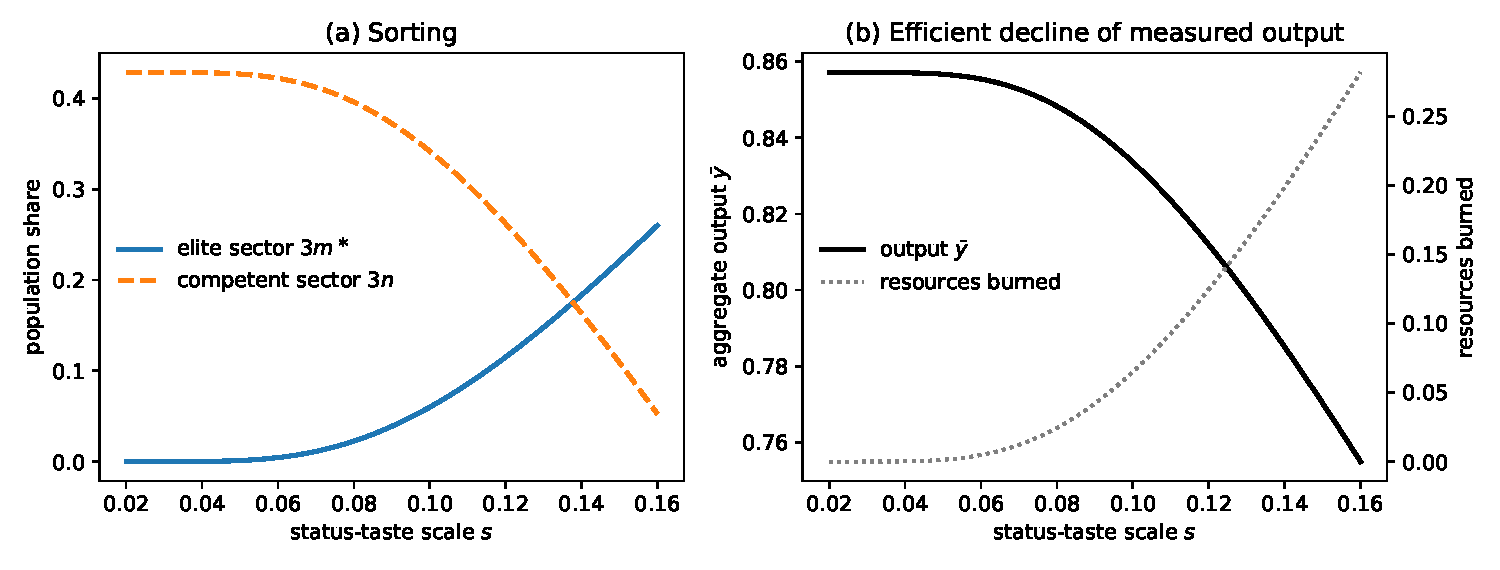
\includegraphics[width=\textwidth]{figures/status_taste_comparative_statics.pdf}
  \caption{Comparative statics in the status-taste scale $s$ ($\eta\sim$
  Exponential, mean $s$). Panel (a): population shares of the elite and competent
  sectors. Panel (b): aggregate output falls and burned resources rise as status
  taste spreads; every equilibrium shown is Pareto optimal
  (Theorem~\ref{thm:nocorrection}). Parameters as in Section~\ref{sec:example}.}
  \label{fig:comparative}
\end{figure}

\section{Positional Status and the Failure of the Welfare Theorem}\label{sec:positional}

To isolate the positional externality, this section returns to the original four-type
group set $G$ of Section~\ref{sec:model}; the portable route $g_5$ is not included.
Theorem~\ref{thm:nocorrection} rests on status being an \emph{absolute} amenity: the elite-manager membership yields utility $(1+\eta)$ regardless of how many others hold it.
But much of what makes status status is scarcity \citep{hirsch1976social,frank1985demand}: a credential everyone holds confers distinction on no one.
This section makes status positional and shows that everything in Theorem~\ref{thm:nocorrection} breaks --- selectively, and in an instructive way.

\subsection{Positional preferences and equilibrium}

Let $m$ denote the aggregate measure of agents holding an elite-manager seat --- a membership with characteristic $\omega_e$, of which the group set of Section~\ref{sec:model} contains exactly one, $m_{4.1}$ --- and replace the status factor $(1+\eta)$ in the utility specification of Section~\ref{sec:model} with
\begin{equation}\label{eq:positional-utility}
  1 + \eta\, v(m),
\end{equation}
where $v:[0,1]\rightarrow(0,1]$ is continuously differentiable with $v'<0$ throughout and $v(0)=1$: the value of eliteness falls as eliteness spreads.
Each agent is negligible and takes $m$ as given.
(The scalar mass $m$ is unsubscripted; membership labels $m_1,m_{3.1},\dots$ always carry subscripts, so no confusion should arise, and in equilibrium $m$ equals the measure of elite managers, the object the fixed point below denotes $m^\ast$.)
Because utility now depends on \emph{other agents'} memberships, preferences violate the assumptions of \citet{ellickson2006organization}: this is a widespread externality in the sense of \citet{noguchizame2006externalities}.
We accordingly define a \emph{positional group equilibrium} as prices $(p,q)$ and a feasible state $(x,\ell)$ satisfying the three conditions of Section~\ref{sec:framework}, where optimization is with respect to preferences \eqref{eq:positional-utility} evaluated at the aggregate elite mass $m$ induced by the state itself.

Crucially, the externality operates at the level of the \emph{class} of elites (the holders of $m_{4.1}$ across all elite firms) not at the level of any single group.
Membership prices internalize composition effects within a group; they have no instrument that spans groups.
This is precisely the gap in the price system that the welfare theorem needs closed, and it is why the failure below is not a defect of the clubs framework but a fact the framework makes visible.

\subsection{Existence, uniqueness, and self-limiting eliteness}

The wages \eqref{eq:wages}, the output price \eqref{eq:p2}, and the elite-firm break-even income $w_E=z$ are untouched by the externality.
The cutoff condition becomes $(1+\eta^\ast v(m))\,\delta_s\delta_m\, w_E = k$, i.e.,
\begin{equation}\label{eq:positional-cutoff}
  \eta^\ast(m) \;=\; \frac{\eta^\ast_0}{v(m)},
\end{equation}
where $\eta^\ast_0 = \mu k/z - 1$ is the cutoff of Section~\ref{sec:equilibrium}.
Consistency of the conjectured mass with sorting requires $m$ to be a fixed point of
\begin{equation}\label{eq:fixedpoint}
  \rho(m) \;\equiv\; 1 - F\!\left(\frac{\eta^\ast_0}{v(m)}\right).
\end{equation}

\begin{proposition}[Positional equilibrium]\label{prop:positional} Under Assumption~\ref{ass:interior} (maintained at the resulting equilibrium configuration), a positional group equilibrium exists and its elite mass is unique: $\rho$ is continuous and weakly decreasing --- strictly wherever positive --- so $\rho(m)-m$ is strictly decreasing and has exactly one root $m^\ast$, which is strictly positive whenever the support of $F$ extends beyond $\eta^\ast_0/v(0)$.
Moreover: (i) if $m^\ast>0$ then $m^\ast < m_0 \equiv 1-F(\eta^\ast_0)$ --- dilution self-limits the elite; (ii) a FOSD shift of $F$ that is strict at the positional cutoff raises $m^\ast$; if in addition the shift's vertical size at the positional cutoff $\eta^\ast_0/v(m^\ast)$ is weakly smaller than at $\eta^\ast_0$ --- as holds for the exponential scale family used in our examples --- then $m^\ast$ rises by strictly less than $m_0$, so positional concerns dampen the expansion of Proposition~\ref{prop:decline}; (iii) all prices, and the equilibrium values of $p_2$, $w_E$, $n$, and $\bar{y}$ given $m^\ast$, are as in Section~\ref{sec:equilibrium}.
\end{proposition}

The qualification in (ii) is substantive, not decorative: because the positional cutoff $\eta^\ast_0/v(m^\ast)$ exceeds $\eta^\ast_0$, a taste shift concentrated between the two cutoffs would move the positional mass and not the baseline mass, reversing the comparison; damping is a property of shifts that do not favor precisely the diluted region.

Part (i) already delivers a result the baseline cannot: eliteness is self-protecting.
Entry of new elite institutions dilutes the very good they sell, so the market itself polices exclusivity: replication alone cannot arbitrage positional status because relative position cannot be replicated by replication.

\subsection{Failure of optimality and of core equivalence}

\begin{proposition}[Inefficiency]\label{prop:inefficiency} If $v$ is strictly decreasing, Assumption~\ref{ass:interior} is maintained at the positional equilibrium, and its elite mass is strictly positive, then the positional group equilibrium is not Pareto optimal, and its state does not belong to the core.
\end{proposition}

The proof (Appendix~\ref{app:positional}) is constructive and exploits the equilibrium's own structure.
Every non-elite agent (laborers, competent managers, leisure-takers) is at reservation utility and indifferent among their activities; so is every marginal elite.
The planner therefore shuts a small mass $dm$ of elite triples and opens competent triples in the ratio that restores material balance in both goods --- a reallocation that is \emph{exactly} feasible because both adjustment directions have zero value at equilibrium prices.
The released laborers and the redeployed leisure-takers are indifferent; the shut firms' managers lose only their near-marginal status surplus, an amount vanishing relative to $dm$ that the remaining elites' first-order de-dilution gain strictly covers through explicit compensation.
But $v(m)$ rises, so every inframarginal elite is strictly better off: a Pareto improvement, executable by the grand coalition, so the state is blocked and core equivalence fails.
The contrast with Theorem~\ref{thm:nocorrection} is exact: there, shutting elite firms had to take status away from people who had paid its price; here, shrinking the elite \emph{creates} status out of scarcity.

\subsection{Over-entry and the membership tax}

At the laissez-faire equilibrium the marginal entrant weighs the private value of elite membership against its price, but ignores the dilution imposed on every inframarginal elite.
Proposition~\ref{prop:inefficiency} already establishes over-entry in the Pareto sense relevant here: a sufficiently small reduction in the elite mass can be combined with compensation to make a positive measure strictly better off and no one worse off.

To quantify the marginal externality, Appendix~\ref{app:positional} studies the one-parameter compensated cutoff family used in that proof and applies an unweighted utilitarian criterion within the family.
Evaluated at the laissez-faire cutoff, the resulting marginal dilution wedge is
\begin{equation}\label{eq:wedge}
  t^\ast \;=\; \left|v'(m^\ast)\right|\, \frac{w_E}{\,1+\eta^\ast v(m^\ast)\,}
  \int_{\eta\geq\eta^\ast}\!\! \eta\, dF(\eta),
\end{equation}
expressed in units of the marginal entrant's income.
The wedge is strictly positive while the laissez-faire entrant's private surplus is zero, so raising the cutoff increases utilitarian surplus locally within this compensated family.
Equation~\eqref{eq:wedge} does not characterize every Pareto-optimal cutoff and is not, by itself, the welfare-maximizing equilibrium tax.

\begin{proposition}[Membership tax]\label{prop:tax}
Let $t\geq0$ be a level tax, denominated in the input good, on each elite-manager membership.
With population mass one and a uniform per-capita rebate $T$, government budget balance requires
\[
  T=tm.
\]
On an interior taxed branch, define
\[
  \eta_t(m,T)
  \equiv
  \frac{1}{v(m)}
  \left[
    \frac{\mu(k+T)}{z(k+T)-t}-1
  \right],
  \qquad z(k+T)>t.
\]
The taxed equilibrium conditions are
\[
  m=1-F\big(\eta_t(m,T)\big),
  \qquad
  T=tm.
\]

(i) At any fixed rebate $T$, the elite-mass map is continuous and weakly decreasing in $m$, strictly wherever positive, and shifts strictly downward with $t$ while the elite mass remains positive.
It therefore has a unique fixed point conditional on $T$.
No general uniqueness claim is made for the joint $(m,T)$ system; the joint equilibrium is unique and $m(t)$ is strictly decreasing in the numerical example.

(ii) The laissez-faire equilibrium exhibits local over-entry in both senses established above: Proposition~\ref{prop:inefficiency} supplies a Pareto-improving reduction in the elite mass, and the utilitarian derivative along the compensated cutoff family is strictly positive and measured by \eqref{eq:wedge}.

(iii) Along any differentiable joint-equilibrium branch through $t=0$ on which $m'(0^+)<0$, government budget balance gives $T'(0^+)=m^\ast$, and
\[
  \frac{d\bar y}{dt}
  =
  \bar y_m\,m'(0^+)
  +
  \bar y_T\,m^\ast
  +
  \bar y_t.
\]
Here $\bar y_m$ is the derivative in Proposition~\ref{prop:decline}, which is negative under \eqref{eq:decline}; $\bar y_T<0$ is the rebate channel; and
\[
  \bar y_t
  =
  \frac{\phi m^\ast}
  {2c+2r+(\mu+2\lambda-3)k}
  >0
\]
is the direct incidence channel.
Output rises if and only if the positive de-entry and direct-incidence channels together dominate the negative rebate channel.
\end{proposition}

The propositions state exactly what is general and what is example-specific.
Under absolute status there is no corrective wedge: the laissez-faire allocation is Pareto optimal, so a tax cannot be justified as a Pareto correction to status consumption.
This does not imply that every possible tax lowers every scalar welfare criterion.

Under positional status, Proposition~\ref{prop:tax}(ii) establishes over-entry along the compensated cutoff family.
It does not establish that every positive membership tax is Pareto improving, that the tax implements the constructive Pareto improvement of Proposition~\ref{prop:inefficiency}, or that output must rise.
Part~(iii) gives the exact output condition: the de-entry and direct-incidence gains must together dominate the rebate's price effect.
The numerical example supplies the additional welfare result.
There, a small tax raises utilitarian welfare and output simultaneously; the three output channels are $+0.0160$, $-0.0063$, and $+0.0037$, for a total of $+0.0134$ (Appendix~\ref{app:positional}).
A taste distribution thin at the cutoff can instead make entry insufficiently responsive for output to rise even though the elite mass falls.

The practical diagnostic offered by the theory is therefore a question about preferences, not waste alone: \emph{is elite status valued in itself, or valued because others lack it?}
Only the second case generates the positional externality and corrective wedge studied here.

\subsection{Numerical continuation}

Continuing the example of Section~\ref{sec:example} with $v(m)=1/(1+\kappa m)$, $\kappa=25$: the elite mass falls from $m_0\approx 0.0200$ to $m^\ast\approx 0.0086$, with $v(m^\ast)\approx 0.82$, so dilution cuts the elite by more than half, and output rises to $\bar{y}\approx 0.847$.
The same FOSD taste shift (the exponential mean rising from $s=0.10$ to $0.11$) that raises the baseline elite mass by $0.0085$ raises the positional mass by only $0.0023$.
Within the one-dimensional tax-and-uniform-rebate policy class studied in the numerical example, utilitarian welfare is strictly increasing at $t=0$ and reaches its maximum at $t^{W}\approx 0.31$ (about $5.4\%$ of the elite manager's net income, and close to the laissez-faire marginal dilution wedge $t^\ast\approx 0.35$); at that tax the elite mass falls to $0.0050$ and output rises further.
Figure~\ref{fig:positional} displays the fixed point and the welfare curve.
All computations are verified in \path{analysis/positional_model.py}.

\begin{figure}[t]
  \centering
  
\includegraphics[width=\textwidth]{figures/positional_tax.pdf}
  \caption{The positional equilibrium. Panel (a): the map $\rho$ of
  \eqref{eq:fixedpoint} is strictly decreasing, giving a unique elite mass
  $m^\ast$, strictly below the non-positional mass $m_0$ (dotted). Panel (b):
  utilitarian welfare as a function of the membership tax $t$ (uniform lump-sum
  rebate); welfare rises for all small taxes --- the signature of over-entry ---
  and peaks at $t^{W}$. Parameters as in Section~\ref{sec:example} with
  $v(m)=1/(1+25m)$.}
  \label{fig:positional}
\end{figure}

\section{Dynamics: Bequests, Status Demand, and Accumulation}\label{sec:dynamics}

The static analysis holds wealth fixed.
This section also uses the original group set $G$, with either the absolute or positional
status specification, and does not add the portable route to the transition map.
Each generation inherits the resources its parents saved, plays that period's club economy
within its lifetime, and bequeaths.
Three questions organize the analysis.
Does the market for elite status expand or contract as an economy grows?
Does the elite sector's resource burn feed back into accumulation?
And what role, if any, does anticipation play when status spending lowers the resources inherited by future generations?

\subsection{The overlapping-generations economy}

Time is discrete, $t=0,1,2,\dots$.
Each period a measure-one generation is born, inherits per-capita resources $k_t$ (the input good), and lives for one productive period within which the schooling-then-employment sequence of the static model unfolds (memberships are dated within the period, as in \citealt{ellickson2006organization}).
Preferences extend \eqref{eq:utility} with a warm-glow bequest made in the \emph{produced} good --- output invested today is the resource base of the next generation:
\begin{equation}\label{eq:olg-utility}
  u \;=\; d(\ell;\eta)\; x_1^{\zeta/2}\, x_2^{\zeta/2}\, b^{\,1-\zeta},
  \qquad \zeta\in(0,1),
\end{equation}
so an agent with net income $w$ spends $(\zeta/2)w$ on each consumption good and $(1-\zeta)w$ on the bequest, and attains indirect utility $d\,w\,\psi(p_2)$, where $\psi(p_2)$ is a price index common to all agents (Lemma~\ref{lem:period}) --- \emph{still linear in net income}.
Every occupational-indifference condition, membership price, the output price \eqref{eq:p2}, the cutoff \eqref{eq:etastar}, and the positional fixed point \eqref{eq:fixedpoint} therefore carry over verbatim at wealth $k_t$; only the competent-sector scale $n$ adjusts for the saving margin, and the within-period allocation converges to the static model as $\zeta\uparrow1$ (Lemma~\ref{lem:period} in Appendix~\ref{app:dynamics}).
The value $\zeta=1$ is a boundary limit, not an element of the maintained dynamic preference domain.
Invested output converts into next-period resources at a rate $\theta>0$ (a constant-returns storage activity, freely operated, whose linearity makes it profitless and ownerless; the input good itself perishes at the period's end), and children inherit the economy-wide average bequest:
\begin{equation}\label{eq:transition}
  k_{t+1} \;=\; \xi(k_t) \;\equiv\; \theta\,(1-\zeta)\,\frac{\bar{w}(k_t)}{p_2(k_t)},
\end{equation}
where $\bar{w}(k)$ is aggregate net income --- endowment plus the value added of the schools and firms that form at wealth $k$.
Uniform inheritance abstracts from within-generation heterogeneity in inheritances (the gift is pooled, so there are no dynasties in the model, only generations); the Galor--Zeira-style interaction of inherited inequality with elite membership is an important extension we defer.

\begin{definition}\label{def:dynamiceq}
Given $k_0>0$, a \emph{dynamic equilibrium} is a sequence of period allocations and prices such that, in every period $t$, the allocation is a group equilibrium of the period economy at wealth $k_t$ and $k_{t+1}$ is given by \eqref{eq:transition}.
The period allocation is:
\begin{enumerate}
\item the interior equilibrium of Lemma~\ref{lem:characterization}, or its positional counterpart, when Assumption~\ref{ass:interior} holds at $k_t$; and
\item the corresponding elite-free interior equilibrium when either
\[
  z(k_t)\leq0,
\]
or
\[
  z(k_t)>0
  \quad\text{and}\quad
  F\!\left(\frac{\mu k_t}{z(k_t)}-1\right)=1.
\]
\end{enumerate}
The second condition covers bounded-support taste distributions for which elite firms could pay a positive manager income but no agent values elite status enough to enter.
Outside these interior and elite-free interior configurations, the dynamic equilibrium is left undefined; the domain $K$ of Proposition~\ref{prop:map} excludes the remaining corner regimes.
\end{definition}

Because preferences \eqref{eq:olg-utility} contain no forward-looking argument, the definition is genuinely recursive: no agent's optimization requires forecasting, and each period's prices depend only on $k_t$.

\begin{proposition}[The transition map]\label{prop:map} Let $K\subset\R_+$ be an interval on which the period equilibrium of Definition~\ref{def:dynamiceq} is well defined (Assumption~\ref{ass:interior} where the elite sector is viable, the elite-free interior configuration under either condition in Definition~\ref{def:dynamiceq}).
Under \eqref{eq:olg-utility} and condition \eqref{eq:decline}, so that the elite sector is inactive near the origin: (i) the within-period allocation at wealth $k_t\in K$ is the club equilibrium of Section~\ref{sec:equilibrium} (or Section~\ref{sec:positional}) at $k_t$; (ii) $\xi$ is continuous on $K$, with $\xi'(0^+)=\theta(1-\zeta)\phi/(c+r)$, and the elite-free map is bounded (diminishing returns operate through the price of investment, $p_2(k)$, which rises with wealth); (iii) if $\theta(1-\zeta)\phi>c+r$, the origin repels, and any interior crossing of the diagonal from above is a steady state, stable whenever $|\xi'|<1$ there.
\end{proposition}

In our parameterization $K$ comfortably contains the steady states and transition paths studied below, each crossing is unique with $|\xi'|<1$, and at substantially higher wealth or taste the interior configuration eventually fails (the competent sector's market-clearing scale reaches zero, and at extreme wealth every type demands the elite path at the candidate prices), at which point the map would have to be extended by the corner regimes, which we do not need.
The recursivity of Definition~\ref{def:dynamiceq} makes the role of anticipation precise.
The path $(k_t)$ generated by \eqref{eq:transition} may be common knowledge, but forecasts of future utility do not enter \eqref{eq:olg-utility}.
Agents optimize their within-period choices and warm-glow gifts at the prices they face; the resulting decline is therefore not a mistaken forecast or a bubble.
Perfect foresight is behaviorally irrelevant here because the baseline preferences contain no forward-looking argument, not because the paper has solved a forward-looking dynastic problem.

Appendix~\ref{app:motive} establishes a conditional invariance result.
Within the degree-one preference class, any factor common to agents cancels from occupational comparisons, so a common savings rule affects the volume of saving and the resulting wealth path but not prices, wages, sorting, or the elite mass at a given $k$ (Proposition~\ref{prop:invariance}).
The proposition does not derive that savings rule from forward-looking altruism and does not establish that the steady-state comparison is invariant across savings motives.
Within the additive pooled-altruism specification, atomistic parents instead free-ride on the aggregate gift and transfer nothing (Proposition~\ref{prop:commons}), which explains the role of direct warm glow in the baseline.
Dynasty-specific transfers with forward-looking parents remain an extension discussed in Section~\ref{sec:discussion}.

\subsection{Status is a luxury}

\begin{proposition}[Luxury]\label{prop:luxury} The elite cutoff $\eta^\ast_0(k)=\mu k/z(k)-1$ is strictly decreasing in $k$ --- and hence the elite mass $m^\ast(k)$ strictly increasing in $k$ wherever the cutoff is interior to the support of $F$ --- if and only if $\alpha(c+r) < \beta c + \tau r$: precisely the resource-productivity condition \eqref{eq:decline} of Proposition~\ref{prop:decline}.
\end{proposition}

The mechanism is instructive.
The elite sector's excess costs --- the school's burn $(\tau-1)r$, the firm's burn $(\beta-1)c$ --- are \emph{fixed} resource costs, while every wage in the economy scales with wealth.
As $k$ grows, the burn shrinks relative to the status discount that finances it, so the marginal entrant needs less taste for status to justify entry: rich societies buy more eliteness not because their preferences differ but because they can better afford the waste.
Below a viability threshold ($z(k)\leq 0$) the elite sector cannot break even at any taste level: in this economy of identical endowments, a society too poor to cover the burn has no market for wasteful status.
(With endowment inequality, a wealthy stratum can sustain such a market at low \emph{average} wealth --- historical markets in offices, commissions, and titles are the obvious examples --- so the proposition is a within-economy comparative static on aggregate wealth holding the distribution fixed.)
No nonhomotheticity is assumed in \emph{preferences}; the luxury property is technological, produced by fixed real resource requirements meeting wages that scale with wealth, and it would attenuate if the elite sector's costs scaled with wealth as well --- an empirical question about the cost structure of elite institutions.
That the operative condition is the same one that makes the elite sector a drag on output is what disciplines the mechanism.

\subsection{The status drag and the spread of taste}

\begin{proposition}[Status drag]\label{prop:drag} At any wealth $k$ at which the elite sector is active,
\[
\operatorname{sign}\frac{\partial \xi}{\partial m^\ast}
=
\operatorname{sign}\big[\alpha(c+r)-(\beta c+\tau r)\big].
\]
Under condition \eqref{eq:decline}, therefore: (i) the transition map lies strictly below the no-elite-sector map wherever the elite is active, so that whenever each map crosses the diagonal once in that region, the steady states are ordered $k^\ast_{\mathrm{elite}} < k^\ast_{\mathrm{none}}$; (ii) a FOSD spread of the status-taste distribution, strict at the relevant cutoffs, lowers $\xi$ pointwise (strictly where the elite is active), and under the same single-crossing proviso strictly lowers the steady state; (iii) under positional status, and for taste shifts satisfying the damping hypothesis of Proposition~\ref{prop:positional}(ii) at the cutoffs corresponding to each wealth level, the pointwise decline of $\xi$ is strictly smaller wherever the elite sector is active.
\end{proposition}

One condition (the elite sector produces less output per unit of resources) now governs all three of the paper's mechanisms: the static output decline (Proposition~\ref{prop:decline}), the luxury property (Proposition~\ref{prop:luxury}), and the dynamic drag (Proposition~\ref{prop:drag}).
In the example every proviso holds, and the three steady states order as the propositions suggest:
$k^\ast_{\mathrm{abs}}<k^\ast_{\mathrm{pos}}<k^\ast_{\mathrm{none}}$.
Within that example, growth makes status affordable, status absorbs resources that would otherwise support accumulation, and the transition converges to a positive steady state below the status-free counterfactual.

Two qualifications matter.
First, Proposition~\ref{prop:map} rules out convergence to the origin within the maintained near-origin regime when $\theta(1-\zeta)\phi>c+r$: the elite sector is inactive there and the origin repels.
This is a local result on the domain $K$, not a global no-collapse theorem for the corner configurations in which the current transition map is undefined.
The running example remains in $K$ and converges to its positive steady state, so collapse does not occur in the economy actually computed.
Second, under the damping hypothesis of Proposition~\ref{prop:positional}(ii), positional dilution reduces the elite mass's response to a taste shift and therefore reduces the pointwise fall in the transition map.
In the example this protection is quantitatively strong; the proposition does not assign that magnitude generally.

On intertemporal welfare we claim less, deliberately.
Within each period, the absolute-status allocation is Pareto optimal given $k_t$ (Theorem~\ref{thm:nocorrection}); but future generations are not parties to any period's core, warm-glow bequests \citep{andreoni1990} internalize the intergenerational margin only partially, and overlapping-generations economies admit dynamic inefficiency of the \citet{diamond1965} type.
We emphasize accordingly that the steady-state comparisons above are statements about \emph{wealth}, not welfare: if the warm-glow path overaccumulates, a lower steady state need not be a worse one.
Whether the equilibrium path is efficient among feasible paths --- and by what criterion, given that the glow itself is a utility flow --- is a question we flag for the sequel rather than resolve here.

\subsection{Numerical continuation}

Continuing the running example with $\zeta=0.8$ (a 20\% bequest share) and $\theta$ calibrated so that the absolute-status steady state is exactly the static example's wealth, $k^\ast=2$: the steady state is stable ($\xi'(k^\ast)=0.17$), with the static example's prices, wages, cutoff, and elite mass reproduced as the steady-state allocation.
The no-elite counterfactual steady state is $2.085$; the positional steady state $2.045$.
As the taste scale rises from $s=0.10$ to $s=0.19$, the absolute-status steady state falls to $1.73$ --- a 16.8\% wealth loss relative to the no-elite benchmark, with the elite sector (managers together with their firms' workers) swelling to about a fifth of the population, while the positional steady state falls only to $1.97$ (a 5.7\% loss).
After a taste shift to $s=0.18$, the transition $2.00\rightarrow1.74\rightarrow1.77\rightarrow1.76$ settles within three generations; the mild oscillation reflects the map's locally negative slope at the new steady state ($\xi'\approx-0.08$): a higher inherited $k$ supports a larger elite, which shrinks the aggregate gift --- the luxury mechanism operating period by period.
Figure~\ref{fig:dynamics} displays the maps and the steady-state decline.
All computations are verified in \path{analysis/dynamic_model.py}.

\begin{figure}[t]
  \centering
  
\includegraphics[width=\textwidth]{figures/dynamics_collapse.pdf}
  \caption{Dynamics. Panel (a): transition maps at baseline taste ($s=0.1$) for
  the no-elite counterfactual and the absolute-status economy, and the
  absolute-status map after a taste spread ($s=0.18$); the marked point is the
  calibrated steady state $k^\ast=2$. Panel (b): stable steady-state wealth as
  the taste scale $s$ rises --- wealth falls more in the absolute-status
  example, while positional dilution makes the decline smaller. Parameters as
  in Sections~\ref{sec:example}
  and~\ref{sec:positional} with $\zeta=0.8$, $\theta=5.141$.}
  \label{fig:dynamics}
\end{figure}

\section{Empirical Content}\label{sec:empirics}

The model was built to explain a pattern, and it returns a set of predictions sharp enough to be wrong.
We collect them here, together with the existing evidence that bears on each.

\textbf{Compensation.}
Corollary~\ref{cor:wages} pairs conspicuous gross salaries with a predicted lower pecuniary position after the full cost of elite education.
It also yields a sharp structural comparative static.
\citet{fockemaugniessenruenzi2017} provide direct evidence of a compensation discount associated with employer prestige, but existing studies do not test the model's joint lifetime comparison between the elite and competent education--career tracks.
The equilibrium gross wage satisfies
\[
-q_{4.1}
=
\alpha p_2\phi-\beta c+(3-2\lambda^e)k-k,
\]
in which $\tau$ does not appear.
An elite-specific increase in the real resource requirement $\tau r$ is therefore absorbed one for one by the status discount and has zero incidence on the elite manager's gross salary.
By contrast, a common increase in the serious-school resource cost $r$ changes the elite gross wage through the firm's revenue at rate $\alpha$, so the prediction concerns an elite-specific cost shock rather than schooling costs generally.

This is not a prediction about an independently chosen posted tuition.
In the model, school budget balance makes the fee $q_2$ equal to the real resources $\tau r$ used to supply the qualification.
In the data, posted tuition, the net price paid by a student, and institutional resources per student can move separately because of aid, subsidies, gifts, endowment spending, cross-subsidies, or changes in institutional margins.
A valid incidence design must therefore isolate an exogenous change in real resources required per elite qualification and verify how much of that change is borne by the student.
A posted-tuition experiment at unchanged institutional resource use does not test this comparative static.

The second prediction concerns the net position: the empirical counterpart of $w_E<w_M$ is that the elite track's causal lifetime earnings gain, net of the private cost actually borne to obtain the qualification, falls below that of the comparison track.
No existing estimate maps cleanly into that object.
Zero pass-through together with an inferior net position would be consistent with compensating utility from status and would narrow the class of explanations, but it would not uniquely identify status; other unmeasured amenities or nonpecuniary returns could generate the same pattern.
The decomposition therefore bounds the status-financed component conditional on the model's mapping.
It does not cap the total observed premium.

\textbf{Qualification portability.}
Proposition~\ref{prop:portability} predicts a threshold rather than a smooth substitution
between credentials.
Functional eligibility alone need not generate entry: below $\varrho_A$, the portable
route is feasible but no type strictly chooses it.
At intermediate recognition, agents with moderate status tastes select the portable route
while the highest-status-taste agents retain the incumbent route; at and above
$\varrho_D$, the portable route strictly dominates the incumbent route.
An empirical implementation therefore needs separate measures of the real conversion cost
$c_R$ and the recognition attached to the alternative qualification, not merely evidence
that employers are legally permitted to hire its holders.
It should also distinguish displacement of the incumbent pedigree from the aggregate
material effect.
The portable route uses fewer resources per chain, but greater recognition can expand
elite-format employment enough to raise total resource use and lower output, as in the
numerical example.
These are comparative statics of the static model; the paper does not claim that
recognition is one-dimensional or exogenous in the data.

\textbf{Firm accounts versus resource accounts.}
In the central configuration, output, revenue, and pay comparisons all flatter the elite sector, and with $\alpha\geq\beta$ (as in our example) productivity comparisons do as well.
Firm accounts do not include the resources used to produce the manager's qualification, and standard aggregate accounts need not identify whether measured educational expenditure produces skill, amenity, or status.
In particular, additional inputs into public and nonprofit education can be recorded as additional educational output even when the accounts contain no independent measure of the qualification's productive content.
The model's resource wedge is therefore not recoverable from firm productivity or aggregate GDP alone.

Within the model, average schooling resources per managerial position filled are
\[
\frac{nr+m^\ast\tau r}{n+m^\ast}.
\]
This is an exact model object and a useful measurement target, not yet a directly observed measure of burn.
Its empirical counterpart requires matching the flow of resources used to produce managerial qualifications to the flow of positions filled by holders of those qualifications.
Identifying the burn further requires a counterfactual: the resource premium over a qualification that supplies the same productive skill without the status component.
If elite firms also differ in inputs and output, the empirical exercise must measure the firm-side terms $(\beta-1)c$ and $(\alpha-1)(c+r)$ as well.
Credential inflation is the resulting increase in resources required to reach a given class of positions; expenditure per student alone does not identify it.
The numerical examples illustrate the mechanism and are not calibrations of these objects.

\textbf{Status as a luxury.}
Proposition~\ref{prop:luxury} predicts that the elite share of the population rises with aggregate wealth, holding tastes and the endowment distribution fixed.
The prediction is a within-economy comparative static, not a cross-country ranking: because our agents share a common endowment, the model's ``poor economy'' is one in which \emph{no one} can cover the burn, whereas historically poor societies with wealthy strata ran flourishing markets in skill-free position (venal offices, purchased commissions, sold degrees) exactly as an endowment-heterogeneous version would predict.
The mechanism the proposition isolates --- a fixed resource burn financed by wages that scale with wealth --- implies that within an economy, growth expands the elite share, and ties that expansion to the same condition that governs the aggregate drag.

\textbf{Distinguishing absolute from positional status.}
The paper's two welfare regimes are observationally similar in a cross-section (wasteful elite institutions persist in both) but differ in their dynamics.
In the positional equilibrium all monetary prices coincide with the absolute-status benchmark (Proposition~\ref{prop:positional}(iii)); dilution operates through quantities, not wages, so the discriminating observable is the elasticity of the elite share to demand shifts.
Positional status implies damped responses, for shifts satisfying the damping hypothesis of Proposition~\ref{prop:positional}(ii), because each entrant erodes the prize; absolute status implies the full one-for-one quantity response.
Historical episodes shifting the demand for elite positions can therefore discipline the operative regime if the demand shift is measured and competing supply, capacity, and selection responses are separately addressed; the response is not a unique identifier by itself.
Within the model, only the positional regime generates the dilution wedge studied in Proposition~\ref{prop:tax}.

\textbf{What the causal evidence can and cannot say.}
The strongest existing designs identify private effects for students near particular admission or attendance margins.
\citet{zimmerman2019elite} uses discontinuities in admission to elite Chilean business programs and finds effects on top incomes and leadership positions concentrated among men from high-tuition private high schools.
\citet{chettydemingfriedman2026} combine comparisons of applicants admitted from and rejected from Ivy-Plus waitlists with a matriculation design conditioning on admission portfolios.
They find substantial effects on upper-tail outcomes and access to elite graduate schools and prestigious firms.
Their large mean-earnings estimate is inferred from the upper-tail results using higher-powered comparisons and additional mapping assumptions; the direct waitlist design is not precise enough to identify mean earnings in levels.

These designs estimate what happens when a marginal student attends one institution rather than another while the surrounding allocation of places and positions remains in place.
With outcomes defined by income rank, entry into prestigious organizations, and other relative attainments, they do not identify what happens to displaced candidates or to aggregate production when the elite sector expands.
They therefore cannot, on their own, distinguish newly created output from a reallocation of access to a fixed set of high-valued positions.
That limitation is specific to the outcomes and equilibrium margin studied, not to causal research designs as such.

The model is consistent with positive private admission effects and, under condition~\eqref{eq:decline}, a nonpositive aggregate output effect of elite-sector expansion.
The evidence does not establish the latter.
Conversely, causal earnings effects larger than plausible private education-cost differentials press against a literal empirical reading of the baseline net-income prediction and indicate quantitatively important channels absent from it.
Scarcity rents are one possible channel in an extension, but the evidence does not identify them separately from skill production, networks, matching, or occupational reallocation.
The aggregate margin is where the model's distinctive empirical question lies and where current evidence is least complete.

\textbf{Magnitudes and measurement.}
The examples above display mechanisms rather than measure their aggregate importance.
The model nevertheless supplies an exact accounting bridge.
At the steady states of Section~\ref{sec:dynamics}, the wealth gap between the elite-active economy and its status-free counterfactual satisfies (Remark~\ref{rem:loss} in Appendix~\ref{app:dynamics})
\[
\frac{k^\ast_{\mathrm{none}}-k^\ast_{\mathrm{elite}}}
     {k^\ast_{\mathrm{none}}}
=
M b,
\]
where
\[
b
\equiv
\frac{
m^\ast(k^\ast_{\mathrm{elite}})
\left[(\tau-1)r+(\beta-1)c\right]
}{
k^\ast_{\mathrm{elite}}
}
\]
is the elite complex's excess resource use relative to the steady-state resource endowment, and $M$ converts that gross resource wedge into a steady-state wealth loss.
The taste distribution enters the identity only through the equilibrium elite mass contained in $b$.
In the running example $M=1.25$, but this is an example-specific value, not a bound: $M$ depends on both the fraction of excess resource use not offset by additional output and the stability margin of the no-elite transition map.

The identity does not authorize substituting an annual education-expenditure share of GDP for $b$.
The denominator of $b$ is the model's inherited resource state $k^\ast_{\mathrm{elite}}$, and one model period is a generation.
Annual educational expenditure is a flow, while GDP is neither defined nor shown to equal that resource state.
A quantitative application therefore requires an explicit temporal and accounting bridge between observed flows and the model's period resource endowment.

Available scale facts remain informative about where measurement should begin.
U.S.\ degree-granting postsecondary institutions spent \$702 billion in 2020--21 \citep{nces2023expenses}, roughly three percent of contemporaneous GDP \citep{bea2022gdp}, but total institutional expenses include activities other than credential production and do not distinguish productive education from status production.
Likewise, the twelve Ivy-Plus colleges enroll roughly $0.8$ percent of U.S.\ college students \citep{chettydemingfriedman2026}.
That student-share denominator is relevant to educational scale, but it is not by itself the share of managerial positions filled through status-intensive qualifications.

A model-consistent magnitude exercise must identify four objects.
First is the share of the relevant flow of managerial positions filled by holders of status-intensive qualifications, the empirical counterpart of $m^\ast/(n+m^\ast)$.
Second is the real resource premium per such qualification over a skill-equivalent alternative, the counterpart of $(\tau-1)r$.
Third is any firm-side excess input net of additional output, represented by $(\beta-1)c$ and $(\alpha-1)(c+r)$.
Fourth is the mapping from these resource flows into the inherited resource state and the no-elite transition slope that determines $M$.
These are the observables and counterfactuals needed to turn the exact identity into a calibration.
Until they are supplied, the identity is a measurement agenda rather than a quantitative estimate of the U.S.\ steady-state wealth loss.

\section{Discussion}\label{sec:discussion}

\textbf{GDP versus welfare.}
Propositions~\ref{prop:coexist}--\ref{prop:decline} and Theorem~\ref{thm:nocorrection} jointly formalize a distinction the public debate conflates: what declines as elite status spreads is real output net of resources burned, a quantity that neither firm accounts nor standard national accounts isolate, and not what agents maximize.
Any diagnosis of ``inefficiency'' from output or TFP data alone presumes status utility does not count --- a normative stance that should be argued, not assumed.

\textbf{Portability and institutional change.}
The portability result identifies a market route to incumbent displacement that does not
require suppressing status demand.
A lower-resource chain can replace an incumbent pedigree once it is both functionally
eligible and sufficiently recognized.
The distinction matters because credential reform that changes formal eligibility without
changing recognition can leave the incumbent untouched, while recognition can generate a
coexistence interval before displacement.
The result remains deliberately reduced form about recognition.
Endogenizing why audiences recognize one route, how recognition diffuses, or how
incumbents defend it would require a reputation or political-economy model not contained
here.

\textbf{Positional scarcity and observed premia.}
The positional model developed here changes quantities but not monetary prices: Proposition~\ref{prop:positional}(iii) leaves $q_{4.1}$ and the compensation decomposition unchanged at any given elite mass.
It therefore does not itself generate a scarcity-rent amplification of elite wages.
An extension in which firms compete for a capped stock of already-qualified elites could generate such rents, but that result would require a separate labor-market mechanism and is not established here.
Accordingly, observed or causal earnings premia larger than the tuition-based component in Corollary~\ref{cor:wages} should be treated as evidence of additional channels --- potentially scarcity, but also skill production, networks, matching, or occupational assignment --- rather than assigned to scarcity by the present model.

\textbf{Extensions.}
Three extensions strike us as most valuable.
First, dynasty-specific inheritance: uniform inheritance isolates the aggregate mechanism, but letting parents bequeath directly to their children would interact inheritance with elite membership in the manner of \citet{galorzeira1993}, and would let the model speak to intergenerational mobility at the top.
The sign is worth stating honestly: because elite managers accept lower \emph{net} incomes, dynasty-specific bequests would transmit less wealth down elite lines --- the status discount is dynastically self-impoverishing --- so the model's persistence is institutional rather than dynastic, and reconciling the two is precisely what the extension is for.
Relatedly, replacing warm glow with forward-looking altruism would introduce an expectation-dependent savings problem.
Under the additive pooled-altruism benchmark of Proposition~\ref{prop:commons}, atomistic parents instead contribute nothing to the common gift; the sign and magnitude of the effect under other altruistic specifications are not established here.
Second, parents who value their children's \emph{status} rather than the bequest itself --- the natural sharpening of the warm-glow specification, which would make elite membership itself heritable in demand.
Third, intertemporal welfare: each period's absolute-status allocation is optimal given its inheritance, but the path's efficiency across generations --- and what, if anything, a generation-spanning planner could improve even in the absolute-status world --- is open, and the answer plausibly differs between the absolute and positional regimes.

\section{Conclusion}\label{sec:conclusion}

This paper shows why a familiar inference about competition can fail.
A resource-intensive elite institution's survival need not reflect weak competition,
market power, or an unpriced cost.
In the model, measurable output is not the complete product: qualification,
organizational membership, and status are also valued, and their buyers finance the
additional resources through a lower net pecuniary position.
Competitive membership prices can therefore support an output-reducing absolute-status
allocation in the strong core that is strongly Pareto optimal.
General equilibrium is essential to this conclusion because the relevant competitive
object is the complete school--career membership chain, not a school production function
viewed in isolation.

The portability result disciplines rather than protects that persistence.
When a lower-resource alternative is functionally portable and sufficiently recognized,
it displaces the incumbent chain; with intermediate recognition, entry precedes
displacement.
Even then, incumbent displacement does not imply elimination of resource-intensive elite
organization, because the cheaper route may expand total demand for elite-format
management.

The positional and dynamic analyses delimit the baseline result.
Positional status creates a dilution externality and permits a welfare-improving tax in
the numerical example.
Under the stated resource-productivity condition, the same institutional resource wedge
propagates into lower accumulation, without establishing a forward-looking dynastic or
intertemporal welfare result.
Empirically, the central distinctions are among productive skill, membership value,
qualification portability, and recognition.
The paper's message is therefore not that resource-intensive elite organization is always
efficient.
It is that competition and efficiency can be assessed only after the complete product,
the incidence of its cost, and the feasibility of rival qualification chains are placed
in equilibrium.

\appendix

\section{Derivations and Proofs}\label{app:derivations}

All computations in this appendix are verified symbolically in
\path{analysis/static_model.py}.

\subsection{Demand and indirect utility}
An agent with net income $w$ solves $\max_{x_1,x_2} d\sqrt{x_1x_2}$ subject to $x_1+p_2x_2=w$, giving $x_1=w/2$, $x_2=w/(2p_2)$, and indirect utility $d\,w/(2\sqrt{p_2})$.

\subsection{Dominated lists}
\begin{lemma}\label{lem:dominated} At any prices satisfying \eqref{eq:prices} with $r,\tau r>0$, every feasible list other than the five in Section~\ref{sec:model} is strictly dominated.
\end{lemma}

\begin{proof}
The consumption sets allow at most one school and at most one job, and a graduate of one school type cannot hold the other type's managerial membership, so the only feasible lists beyond the five are schooling with no job and schooling combined with a laborer job.
(i) Schooling with no job yields taste factor $d\leq\delta_s<1$ and net income $k-q_j<k$, dominated by leisure.
(ii) Schooling plus a laborer job multiplies the laborer's taste factor by $\delta_s<1$ and subtracts tuition, dominated by the same laborer job alone.
\end{proof}

\subsection{Proof of Lemma~\ref{lem:characterization}}
\emph{Budget balance.}
Schools: $q_1-r=0$, $q_2-\tau r=0$ by \eqref{eq:prices}.
Competent firms: $q_{3.1}+2q_{3.2} - c + p_2\phi = (k-r-\mu k) + 2(k-\lambda k) - c + p_2\phi = 0$ by \eqref{eq:p2}.
Elite firms: $q_{4.1}+2q_{4.2} - \beta c + p_2\alpha\phi = 0$ reduces, using \eqref{eq:p2}, to $w_E = z$, which is \eqref{eq:etastar}.
\emph{Optimization.}
By Lemma~\ref{lem:dominated} only the five vocational choices need comparison; by construction of \eqref{eq:wages} and \eqref{eq:cutoff}, types below $\eta^\ast$ are indifferent among the four non-elite choices and strictly prefer them to the elite path, types above strictly prefer the elite path, and the marginal type is indifferent.
\emph{Consistency and material balance.}
The stated measures fill every group type in the required proportions; market clearing \eqref{eq:clearing} solves
\begin{equation}\label{eq:nclosed}
  n \;=\; \frac{k - (1-3m^\ast)\frac{k}{2} - m^\ast\left[\frac{w_E}{2} +
  w_{L^\ast} + \tau r + \beta c\right]}
  {\frac{w_M}{2} + w_L - \frac{3k}{2} + r + c},
\end{equation}
positive under Assumption~\ref{ass:interior}.
\emph{Walras.}
Substituting \eqref{eq:nclosed} and \eqref{eq:etastar} into the $y_2$ market, demand $\sum \text{(measures)}\times w/(2p_2)$ equals supply $\phi(n+\alpha m^\ast)$ identically (machine-verified).
Uniqueness of the interior configuration follows because, when a positive measure of agents also holds the empty list, indifference with leisure and budget balance imply \eqref{eq:wages}--\eqref{eq:etastar}, and \eqref{eq:nclosed} is linear in $n$.
\qed

\subsection{Proof of Proposition~\ref{prop:coexist}} Subtracting the two firm budget-balance conditions, $p_2\phi(1-\alpha) = (w_M - w_E) - 2(w_{L^\ast}-w_L) - (\beta-1)c - (\tau-1)r$ after substituting \eqref{eq:prices}; the left side is positive iff $\alpha<1$, given $p_2>0$.
\qed

\subsection{Proof of Proposition~\ref{prop:decline}} $\eta^\ast$ solves \eqref{eq:etastar}, which contains no object depending on $F$; a FOSD shift weakly raises $1-F(\eta)$ pointwise, and strictness at $\eta^\ast$ raises $m^\ast=1-F(\eta^\ast)$ strictly.
Differentiating $\bar{y}=\phi(n+\alpha m^\ast)$ with $n$ from \eqref{eq:nclosed} gives
\[
\begin{aligned}
\frac{d\bar{y}}{dm^\ast}
&=\phi\left(\alpha-1+\frac{d(n+m^\ast)}{dm^\ast}\right),\\
\operatorname{sign}\frac{d\bar{y}}{dm^\ast}
&=\operatorname{sign}\big[\alpha(c+r)-(\beta c+\tau r)\big].
\end{aligned}
\]
Direct computation gives the sharper identity
\[
\frac{d\bar{y}}{dm^\ast}
=
\frac{\phi\,[\alpha(c+r)-(\beta c+\tau r)]}
{2c+2r+(\mu+2\lambda-3)k},
\]
whose denominator is positive (machine-verified in
\path{analysis/static_model.py}).
\qed

\section{Verification of Framework Assumptions}\label{app:assumptions}

\emph{Consumption sets.}
$X_a = \R^2_+\times\Lists_a$ with $\Lists_a$ the lists satisfying the schooling prerequisites and the at-most-one-school, at-most-one-job bounds; the list bound is $\bar\ell=2$.
Free upward disposal in private goods holds.
The correspondence $a\mapsto X_a$ is constant in $a$ (types differ only through $u$), hence measurable.

\emph{Utility.}
$u(x,\ell;\eta)$ is continuous and jointly measurable since $\eta\mapsto d(\ell;\eta)$ is continuous and $a\mapsto\eta_a$ is measurable.
For each fixed list it is strictly increasing on the interior of $\R^2_+$ and locally nonsatiated everywhere on $\R^2_+$.
Although $h=\sqrt{x_1x_2}$ is constant when movement is confined to an axis, adding an arbitrarily small strictly positive amount of both goods strictly raises utility from every boundary bundle.
This is the boundary property used in the direct proof of Theorem~\ref{thm:nocorrection}; no appeal to a strict-monotonicity assumption or to the desirable-endowment implication of the external welfare theorem is required.

\emph{Existence.}
Lemma~\ref{lem:characterization} exhibits the interior equilibrium used in the static analysis directly.
Definition~\ref{def:dynamiceq} restricts the dynamic analysis to wealth levels at which either that configuration or the corresponding elite-free interior configuration is well defined.
No general existence claim is made here for the remaining corner configurations.

\section{Displacement: Proofs}\label{app:displacement}

The openness computations of part (ii) are verified in
\path{analysis/displacement_theorem.py}.

\subsection{Part (i), core route}
Let $(x,\ell)$ be feasible with $\nu(g)>0$, and let $S$ be the assumed positive-measure set of agents consuming strictly positive bundles.
We exhibit a strong block by the grand coalition.
Assign to every agent the list $\hat\ell_a=\ell_a[g\rightarrow g']$; clause (E1) preserves individual feasibility, and the substitution preserves list lengths, so the bound $\bar\ell$ is respected.
Consistency holds because the seats released from type-$g$ groups fill type-$g'$ groups in exactly the required proportions (the profiles coincide): $\hat\nu(g')=\nu(g')+\nu(g)$, $\hat\nu(g)=0$, and all other masses are unchanged.
Aggregate net output changes by $\nu(g)(y'-y)\geq 0$, $\neq 0$; choose a good $j$ with $y'_j>y_j$ and distribute the released surplus $\nu(g)(y'_j-y_j)>0$ of good $j$ uniformly across agents, which free upward disposal keeps inside every consumption set.
By (E2) the substitution leaves every agent's utility unchanged, the added goods leave almost every agent weakly better off, and every agent in $S$ is strictly better off, utility being strictly increasing at interior bundles.
This is a strong block: the state is not in the strong core.
The equilibrium exclusion follows independently from the pricing route below.
The equilibria of Lemma~\ref{lem:characterization} satisfy the proviso: almost every agent's net income is strictly positive (leisure-takers have $w=k>0$ and elite managers $w_E=z>0$ by Assumption~\ref{ass:interior}(i); $z<k$ is possible within Assumption~\ref{ass:interior}, so the argument uses positivity, never size), and demand is then interior.

\subsection{Part (i), pricing route}
Consider any group equilibrium in which a positive measure of agents consumes an interior bundle; as just verified, the equilibria of Lemma~\ref{lem:characterization} qualify, and so do their positional counterparts, whose prices coincide (Proposition~\ref{prop:positional}(iii)).
\emph{Step 1: goods prices are strictly positive.}
Were some $p_j=0$, an agent in the interior set could add the free good at unchanged expenditure and be strictly better off, contradicting optimization.
\emph{Step 2: the seat bundles are ordered.}
Budget balance holds for every type in the augmented group set $G^+$, active or not, so subtracting the two conditions gives $\sum_{\omega}\pi(\omega)\left[q(\omega,g)-q(\omega,g')\right] = p\cdot(y'-y) > 0$ by Step 1.
\emph{Step 3: arbitrage.}
Suppose $\nu(g)>0$.
Integrating the saving from full-list substitution over the population, $\int \left[q\cdot\ell_a - q\cdot\ell_a[g\rightarrow g']\right]d\iota = \nu(g)\,p\cdot(y'-y)>0$, so a positive-measure set of agents each realizes a strictly positive saving from substituting her own list.
For any such agent the choice (substituted list, current bundle plus a strictly positive amount of every good purchased with the saving) is feasible by (E1), affordable, and strictly preferred: her taste factor is strictly positive, so an interior bundle beats a boundary bundle, and strict monotonicity does the rest when her bundle was already interior.
This contradicts optimization; hence $\nu(g)=0$.
The argument never exchanges a single seat in isolation --- the saving is evaluated on the whole list, which is what (E1)--(E2) license --- and in the positional regime it proceeds at fixed elite mass, since the substitution preserves the set of agents holding $\omega_e$ seats and the status factors of Section~\ref{sec:model} attach to characteristics, not to membership objects.

\subsection{Part (ii)}
At the parameters of Section~\ref{sec:example}, Assumption~\ref{ass:interior} holds with strict inequalities ($z=5.75\in(0,\mu k)=(0,8)$, $n\approx 0.114>0$, $\sigma_0\approx 0.598>0$).
Every equilibrium object is a closed-form continuous function of the parameter vector, so the strict inequalities persist on an open neighborhood, on which Lemma~\ref{lem:characterization} delivers the active-elite equilibrium and Theorem~\ref{thm:nocorrection} places its state in the strong core.
The dominance and equivalence clauses are parameter-free on the neighborhood: $y_{g_1}=(-r,0)\geq(-\tau r,0)=y_{g_2}$ strictly for $\tau>1$, with the common profile $\pi_1$; both schools carry the amenity factor $\delta_s$, so (E2) holds on the common feasible domain; and (E1) fails at the elite manager's list, $\{m_2,m_{4.1}\}\in X_a$ while $\{m_1,m_{4.1}\}\notin X_a$, because the serious school does not confer $\omega_e$.
No other pair of types shares a profile ($\pi_3$ demands $\omega_e$ where $\pi_2$ demands $\omega_m$), so no other type in $G$ is membership-equivalent to either elite type.
The companion script verifies the neighborhood claim numerically: all conditions hold on a $\pm 3\%$ one-at-a-time grid and under $20{,}000$ random joint $\pm 1.5\%$ perturbations, with per-parameter symmetric margins of $\pm 4\%$ ($\alpha$), $\pm 7\%$ ($\lambda,\lambda^{e}$), and at least $\pm 10\%$ (all others).
The binding constraint as $\alpha$ rises is interiority ($n>0$), not the dominance inequality: coexistence is robust, and what limits the neighborhood is exactly Assumption~\ref{ass:interior}.
\qed

\begin{remark}[The proviso is vacuous in our economy]\label{rem:proviso}
In any group equilibrium of the economy of Section~\ref{sec:model}, or of an admissible augmentation considered in Theorem~\ref{thm:displacement}, both goods prices are strictly positive, so the interiority proviso of part~(i) excludes nothing.
If $p_2=0$, then $p_1>0$ (prices are nonzero), every agent's wealth $p_1k$ is strictly positive, and any agent can afford a bundle she strictly prefers to any candidate optimum --- her endowment's worth of the input good together with an arbitrarily large amount of the free consumption good --- violating optimization.
If $p_1=0$, every agent's wealth is zero, while budget balance for the competent firm gives $q_{3.1}+2q_{3.2}=-p_2\phi<0$, so some seat carries a strictly negative price; schooling is free ($q_1=p_1r=0$), so the seat is attainable, and its wage funds an interior bundle at nonpositive total cost --- a strictly preferred affordable choice, violating optimization.
Hence $p\gg 0$; every agent's wealth is then strictly positive, every taste factor is strictly positive, and almost every agent's chosen bundle is interior.
The hypotheses of both proof routes therefore hold at every group equilibrium of our economy, and the summaries in the text may read ``every equilibrium'' without qualification.
\end{remark}

\section{Portable Qualifications: Proofs}\label{app:portability}

The algebra and the numerical continuation in this section are verified in
\path{analysis/portability_extension.py}.

\subsection{Proof of Proposition~\ref{prop:portability}}

\emph{Prices and occupational indices.}
Budget balance for $g_5$ follows from \eqref{eq:portable-prices} and budget balance for
$g_4$:
\[
\begin{aligned}
q_{5.1}+2q_{5.2}-(\beta c+c_R)+p_2\alpha\phi
&=(q_{4.1}+c_R)+2q_{4.2}-(\beta c+c_R)+p_2\alpha\phi\\
&=0.
\end{aligned}
\]
The portable manager's net income is
\[
k-r-q_{5.1}
=k-r-q_{4.1}-c_R
=z+(\tau-1)r-c_R
=z+D.
\]
Every nonelite occupation delivers utility index $\mu k$ after multiplication by
$2\mu\sqrt{p_2}$; the incumbent and portable elite paths then give the two affine
indices in \eqref{eq:portable-indices}.

\emph{Threshold ordering.}
Under \eqref{eq:portable-interior-income},
\[
\frac{\varrho_A}{\varrho_D}
=
\frac{\mu k-(z+D)}{\mu k-z}
\in(0,1),
\]
so $0<\varrho_A<\varrho_D<1$.
The incumbent and portable indices cross, when $\varrho<\varrho_D$, at
\[
\eta_{EP}
=
\frac{D}{z-\varrho(z+D)}.
\]
The portable index crosses the nonelite index, for $\varrho>0$, at
\[
\eta_P
=
\frac{\mu k-(z+D)}{\varrho(z+D)}.
\]
Direct subtraction gives
\[
\eta_{EP}-\eta_P
=
\frac{(\mu k-z)(z+D)(\varrho-\varrho_A)}
{\varrho(z+D)[z-\varrho(z+D)]}.
\]
The denominator is positive for $0<\varrho<\varrho_D$, so the sign is the sign of
$\varrho-\varrho_A$.
At $\varrho=\varrho_A$, the two crossings coincide with
$\eta_E=\mu k/z-1$; all three indices meet at that single type.

For $\varrho<\varrho_A$, the portable line crosses the incumbent line before the
incumbent reaches the nonelite index and crosses the nonelite line, if at all, only after
the incumbent is already above it.
It is therefore never strictly on the upper envelope.
For $\varrho_A<\varrho<\varrho_D$, the ordering
$\eta_P<\eta_{EP}$ gives the three intervals stated in the proposition.
For $\varrho\geq\varrho_D$, the portable line has a strictly higher intercept,
$z+D>z$, and a weakly greater slope,
$\varrho(z+D)\geq z$, so it strictly dominates the incumbent line at every $\eta$.
This proves the sorting claims and \eqref{eq:portable-masses}.
If the support of $F$ ends below $\eta_{EP}$, the formal upper interval contains no
agents and the incumbent route disappears before the distribution-free dominance
threshold; this proves the bounded-support qualification.

\emph{Consistency and goods markets.}
Let $m=m_E+m_P$.
The masses $m_E$ and $m_P$ fill the manager seats of $g_4$ and $g_5$ and require
$2m_E$ and $2m_P$ elite-condition laborers.
The competent sector contains $n^P$ managers and $2n^P$ laborers.
The remaining mass
\[
\sigma_0^P=1-3n^P-3m
\]
holds the empty list.
The agents outside the two elite-manager intervals have total mass
$1-m=3n^P+2m+\sigma_0^P$, exactly the mass needed for the nonelite managerial,
labor, and leisure assignments.
Because those agents are indifferent among the relevant nonelite choices and the
population is nonatomic, they can be assigned measurably to fill all seats.

Input-good clearing is
\[
\begin{aligned}
k
={}&
\sigma_0^P\frac{k}{2}
+m_E\frac{z}{2}
+m_P\frac{z+D}{2}
+2(m_E+m_P)\frac{\lambda^e k}{2}\\
&+n^P\frac{\mu k}{2}
+2n^P\frac{\lambda k}{2}
+m_E(\tau r+\beta c)
+m_P(r+\beta c+c_R)
+n^P(r+c).
\end{aligned}
\]
Substituting $\sigma_0^P=1-3(n^P+m_E+m_P)$, then using
\eqref{eq:p2}, \eqref{eq:Z}, and \eqref{eq:portable-advantage}, reduces this equation
to \eqref{eq:portable-clearing}.
The consumption-good market clears by Walras' law.

\emph{Optimization and existence.}
In the augmented consumption sets the only new undominated managerial list is
$\{m_1,m_{5.1}\}$.
The two elite-condition labor memberships $m_{4.2}$ and $m_{5.2}$ are distinct objects
but have identical utility and net income under \eqref{eq:portable-prices}; schooling
without managerial employment and schooling combined with labor remain strictly
dominated by the same arguments as Lemma~\ref{lem:dominated}.
The upper-envelope calculation therefore establishes optimization over every feasible
list.
Budget feasibility follows from the Cobb--Douglas demands at each route's net income.
Together with budget balance, consistency, and goods-market clearing, this proves
existence whenever $n^P>0$ and $\sigma_0^P>0$.
Strict sorting away from the cutoff types and the linear clearing equation give the
stated uniqueness on the interior branch.

\emph{Comparative statics.}
In the coexistence region,
\[
\frac{d\eta_P}{d\varrho}
=
-\frac{\mu k-(z+D)}{\varrho^2(z+D)}
<0,
\qquad
\frac{d\eta_{EP}}{d\varrho}
=
\frac{D(z+D)}{[z-\varrho(z+D)]^2}
>0.
\]
Strict increase of $F$ on its support then implies that $m_P$ and
$m_E+m_P=1-F(\eta_P)$ rise while $m_E=1-F(\eta_{EP})$ falls.
\qed

\subsection{Proof of Corollary~\ref{cor:chain-displacement}}

The price-support proof of Theorem~\ref{thm:nocorrection} applies without change to
$G^P$.
It uses only agent optimization, consistency, material feasibility, budget balance for
every available group type, strictly positive goods prices, and the private-goods
boundary property verified in Appendix~\ref{app:assumptions}.
All are satisfied by the equilibria of Proposition~\ref{prop:portability}.
Their states therefore lie in the strong core and are strongly Pareto optimal.

For the full-recognition conclusion, set $\varrho=1$ and suppose a candidate state
activates a positive mass $a>0$ of incumbent elite career chains.
At positive prices, attending $g_2$ without taking the associated manager membership is
strictly dominated, while $m_{4.1}$ requires $m_2$; hence equal masses of $g_2$ schools
and $g_4$ firms serve those managers.
Replace those masses by $a$ groups of type $g_1$ and $a$ groups of type $g_5$.
Each incumbent manager exchanges the list $\{m_2,m_{4.1}\}$ for
$\{m_1,m_{5.1}\}$, and each of the associated laborers exchanges $m_{4.2}$ for
$m_{5.2}$.
The new lists are feasible and consistent.
At $\varrho=1$ the affected managers and laborers receive exactly the same membership
utility as before, and the replacement produces the same amount $\alpha\phi$ of the
consumption good.
Its input requirement is smaller by
\[
(\tau r+\beta c)-(r+\beta c+c_R)
=D>0
\]
per career chain.
Distributing the released input good across agents with positive private-goods
consumption makes a positive-measure set strictly better off and no one worse off.
The candidate state is therefore strongly blocked.

Every group-equilibrium state of the augmented absolute-status economy satisfies the
same direct price-support argument and hence belongs to the strong core, so no such
equilibrium can activate the incumbent chain.
\qed

\subsection{Derivation of the output identity}

Equation~\eqref{eq:portable-clearing} gives
\[
n^P
=
\frac{k
-m_E(\tau r+\beta c+\alpha p_2\phi)
-m_P(r+\beta c+c_R+\alpha p_2\phi)}
{c+r+p_2\phi}.
\]
Substitute this expression into
$\bar y^P=\phi[n^P+\alpha(m_E+m_P)]$ and collect the coefficients on
$m_E$ and $m_P$.
The result is \eqref{eq:portable-output}.
Equation~\eqref{eq:portable-burn} is the corresponding direct comparison of each
elite-format chain's input requirement with the competent chain's requirement $r+c$.

\section{Positional Extension: Proofs}\label{app:positional}

All computations are verified in \path{analysis/positional_model.py}.

\subsection{Proof of Proposition~\ref{prop:positional}} The occupational-indifference conditions for non-elite choices do not involve $m$, so \eqref{eq:wages} and \eqref{eq:p2} are unchanged, as is the elite break-even income $w_E=z$ from firm budget balance.
The cutoff type solves $(1+\eta v(m))\,\delta_s\delta_m w_E = k$, giving \eqref{eq:positional-cutoff}; sorting is strict above and below the cutoff because \eqref{eq:positional-utility} is strictly increasing in $\eta$ for fixed $m$.
Consistency of $m$ with sorting is \eqref{eq:fixedpoint}.
Since $v$ is continuous and strictly decreasing and $F$ is continuous and strictly increasing on its support, $\rho$ is continuous and weakly decreasing --- strictly wherever $\rho>0$; when $F$ has bounded support, $\rho$ vanishes identically for $m$ large enough that $\eta^\ast_0/v(m)\geq\bar\eta$.
Hence $\rho(m)-m$ is continuous and strictly decreasing with $\rho(0)-0=1-F(\eta^\ast_0)$ and $\rho(1)-1<0$, so it has exactly one root $m^\ast\in[0,1)$; $m^\ast>0$ iff $\rho(0)>0$, i.e., iff the support of $F$ extends beyond $\eta^\ast_0=\eta^\ast_0/v(0)$.
(i) Since $v(m^\ast)<1$ for $m^\ast>0$, $\eta^\ast=\eta^\ast_0/v(m^\ast)>\eta^\ast_0$, so $m^\ast=1-F(\eta^\ast)<1-F(\eta^\ast_0)=m_0$.
(ii) Replacing $F$ by $\tilde F\leq F$ shifts $\rho$ up pointwise, strictly at $m^\ast$ if the shift is strict at the positional cutoff; with $\rho-\mathrm{id}$ strictly decreasing, the root rises strictly.
The baseline mass rises by $\Delta m_0 = F(\eta^\ast_0)-\tilde F(\eta^\ast_0)$, while the positional mass rises by at most the vertical shift of $\rho$ at the old fixed point, $\Delta\rho(m^\ast) = F(\eta^\ast_0/v(m^\ast))-\tilde F(\eta^\ast_0/v(m^\ast))$, because the movement along the strictly decreasing $\rho-\mathrm{id}$ can only shrink the vertical displacement.
When the shift satisfies $\Delta\rho(m^\ast)\leq\Delta m_0$ --- the hypothesis of (ii), which holds for the exponential scale family with means $s'>s$, since its vertical shift $e^{-\eta/s'}-e^{-\eta/s}$ is decreasing in $\eta$ beyond a threshold below the relevant cutoffs --- the positional increase is strictly smaller.
(iii) Immediate, since given $m^\ast$ the remaining conditions coincide with those of Lemma~\ref{lem:characterization}.
\qed

\subsection{Proof of Proposition~\ref{prop:inefficiency}} Work at the equilibrium of Proposition~\ref{prop:positional}.
Shutting one elite triple and moving its three members to leisure at their reservation utility changes aggregate excess demand by $(a_e,b_e)$ in (input, output): \[ a_e = \tau r + \beta c + \tfrac{w_E}{2} + w_{L^\ast} - \tfrac{3k}{2},
\qquad
b_e = -\alpha\phi + \frac{w_E + 2w_{L^\ast} - 3k}{2p_2}, \] and elite-firm budget balance implies $a_e + p_2 b_e = 0$.
Opening one competent triple staffed from the (indifferent) leisure pool changes excess demand by $(-a_c, b_c)$ with $a_c = c + r + (w_M+2w_L-3k)/2$, $b_c = \phi - (w_M+2w_L-3k)/(2p_2)$, and competent budget balance implies $a_c = p_2 b_c$.
Both vectors are orthogonal to $(1,p_2)$, hence collinear; moreover $a_e = \tfrac12(\tau r+\beta c+\alpha p_2\phi)>0$ and $a_c = \tfrac12(c+r+p_2\phi)>0$ (both identities machine-verified), so shutting mass $dm>0$ of elite triples and opening $dn = (a_e/a_c)\,dm>0$ competent triples restores material balance in both goods \emph{exactly}, and Assumption~\ref{ass:interior}(iv) ($\sigma_0>0$) supplies the leisure pool from which the $3\,dn$ additional competent-sector members are drawn at reservation utility.
Two groups of agents require care.
Non-elite agents, and the laborers released from the shut elite firms, are indifferent across all their activities at equilibrium prices, so their reassignment is utility-neutral.
The shut firms' \emph{managers} --- types $\eta\in(\eta^\ast,\eta_{dm})$, where $F(\eta_{dm})-F(\eta^\ast)=dm$ --- are not: each strictly preferred elite membership, with an individual surplus that vanishes as $\eta\downarrow\eta^\ast$, so aggregate mover surplus is $o(dm)$ while the de-dilution gain to the $m^\ast-dm$ remaining elites is of order $dm$.
Compensate each mover with a goods transfer equal to her forgone surplus, financed pro rata by the remaining elites: for $dm$ small the total compensation is $o(dm)$, the elites' first-order gain $\eta\,[v(m^\ast-dm)-v(m^\ast)]\,\delta_s\delta_m w_E\,h_0>0$, where $h_0\equiv 1/(2\sqrt{p_2})$, strictly covers it, and every mover is exactly indifferent.
Finally, transfer an arbitrarily small additional amount of each good from the (strictly better off) elites to all agents pro rata: by continuity the elites remain strictly better off, and strict monotonicity on the interior makes almost every agent strictly better off.
The resulting state is feasible and strictly Pareto dominates the equilibrium state; the grand coalition can implement it, so the state is blocked and not in the core.
\qed

\subsection[The compensated utilitarian cutoff family and membership tax]{The compensated utilitarian cutoff family, the wedge \eqref{eq:wedge}, and Proposition~\ref{prop:tax}}

Consider the one-parameter family of feasible states indexed by the cutoff $\hat\eta$ and constructed as in the proof of Proposition~\ref{prop:inefficiency}: non-elite agents are held at reservation utility, displaced managers are compensated for their marginal surplus, and material balance is restored through the competent-sector margin.
Write
\[
  m(\hat\eta)=1-F(\hat\eta),
  \qquad
  h_0\equiv\frac{1}{2\sqrt{p_2}},
\]
and let
\[
  U(\eta,\hat\eta)
  =
  \big[1+\eta v(m(\hat\eta))\big]
  \delta_s\delta_m w_E h_0
\]
be the utility of an elite manager.
Reservation utility is $U_0=kh_0$.
Within this family, changes in unweighted utilitarian welfare are therefore represented by aggregate elite surplus
\[
  \mathcal S(\hat\eta)
  =
  \int_{\hat\eta}^{\infty}
  \big[U(\eta,\hat\eta)-U_0\big]\,dF(\eta).
\]
Using $m'(\hat\eta)=-F'(\hat\eta)$ gives
\[
\begin{split}
  \mathcal S'(\hat\eta)
  ={}&
  -\big[U(\hat\eta,\hat\eta)-U_0\big]F'(\hat\eta)\\
  &+
  F'(\hat\eta)\left|v'(m(\hat\eta))\right|
  \delta_s\delta_m w_Eh_0
  \int_{\hat\eta}^{\infty}\eta\,dF(\eta).
\end{split}
\]
At an interior utilitarian optimum within this family, the marginal type's surplus over reservation utility equals the second term divided by $F'(\hat\eta)$.
Converting that surplus to income units gives
\[
  \left|v'(m(\hat\eta))\right|
  \frac{w_E}{1+\hat\eta v(m(\hat\eta))}
  \int_{\hat\eta}^{\infty}\eta\,dF(\eta).
\]
At the laissez-faire cutoff the marginal surplus is zero.
Evaluating the preceding expression at $(\eta^\ast,m^\ast)$ gives \eqref{eq:wedge}, and $\mathcal S'(\eta^\ast)>0$.
This establishes local utilitarian over-entry along the compensated family.
It does not characterize all Pareto optima; the separate Pareto claim is Proposition~\ref{prop:inefficiency}.

For Proposition~\ref{prop:tax}, let $K\equiv k+T$.
At a fixed rebate, the non-elite reservation incomes and prices are those of the baseline economy evaluated at $K$.
Elite-firm budget balance supplies pre-tax income $z(K)$, so the elite manager's after-tax income is
\[
  w_E^t=z(K)-t.
\]
The positional cutoff and fixed-point map are
\[
  \eta_t(m,T)
  =
  \frac{1}{v(m)}
  \left[
    \frac{\mu K}{z(K)-t}-1
  \right],
  \qquad
  \rho_{t,T}(m)
  =
  1-F\big(\eta_t(m,T)\big).
\]
Government budget balance is
\[
  T=tm.
\]
For fixed $T$, $\rho_{t,T}$ is continuous and weakly decreasing in $m$, strictly wherever positive, and shifts downward as $t$ rises while $z(K)>t$.
Thus its fixed point is unique conditional on $T$ and decreases strictly with $t$ while positive.
The endogenous-rebate equilibrium solves the joint system
\[
  m=\rho_{t,T}(m),
  \qquad
  T=tm.
\]
The proposition makes no general joint-uniqueness claim.
In the numerical example the companion script verifies a unique joint solution with $m(t)$ strictly decreasing.

The over-entry statement in part~(ii) combines Proposition~\ref{prop:inefficiency} with the utilitarian-family derivative derived above.
The wedge \eqref{eq:wedge} is the laissez-faire marginal dilution wedge, not a universal Pareto condition or the welfare-maximizing equilibrium tax.

For part~(iii), consider a differentiable joint-equilibrium branch through $t=0$ and write output as $\bar y(m,T,t)$.
Since $T=tm$,
\[
  T'(0^+)=m^\ast.
\]
The chain rule gives
\[
  \left.\frac{d\bar y}{dt}\right|_{0^+}
  =
  \bar y_m m'(0^+)+\bar y_Tm^\ast+\bar y_t,
\]
with all partial derivatives evaluated at laissez faire.
The mass derivative is
\[
  \bar y_m
  =
  \frac{\phi[\alpha(c+r)-\beta c-\tau r]}
  {2c+2r+(\mu+2\lambda-3)k},
\]
the identity from Proposition~\ref{prop:decline}.
Differentiating market clearing in the rebate gives $\bar y_T<0$.
At fixed mass and rebate, the tax reduces the elite manager's disposable income one for one, releasing input-good consumption to production, so
\[
  \bar y_t
  =
  \frac{\phi m^\ast}
  {2c+2r+(\mu+2\lambda-3)k}>0.
\]
Under \eqref{eq:decline}, the de-entry term is positive whenever $m'(0^+)<0$.
The two positive channels need not dominate the rebate channel, which is why the proposition states a conditional output result.
In the example the three channels are $+0.0160$, $-0.0063$, and $+0.0037$, summing to $+0.0134$.

Utilitarian welfare under the equilibrium tax requires the full general-equilibrium calculation rather than the dilution wedge alone.
In the example,
\[
  \left.\frac{dW}{dt}\right|_{0^+}=0.00125,
\]
of which the de-dilution component accounts for $0.00058$.
The global utilitarian-welfare-maximizing tax is $t^W\approx0.31$, while the laissez-faire dilution wedge is approximately $0.35$; both are computed in \path{analysis/positional_model.py}.
\qed

\section{Dynamics: Proofs}\label{app:dynamics}

All computations are verified in \path{analysis/dynamic_model.py}.

\begin{lemma}[Period equivalence]\label{lem:period} Under preferences \eqref{eq:olg-utility}, an agent with net income $w$ facing $p_2$ chooses $x_1=(\zeta/2)w$, $p_2x_2=(\zeta/2)w$, $p_2b=(1-\zeta)w$, and attains indirect utility $d\,w\,\psi(p_2)$, where $\psi(p_2)\equiv(\zeta/2)^{\zeta}(1-\zeta)^{1-\zeta}p_2^{-(1-\zeta/2)}$ is a price index common to all agents.
Hence all occupational-indifference conditions, membership prices \eqref{eq:prices}, the output price \eqref{eq:p2}, the cutoff \eqref{eq:etastar}, and the positional fixed point \eqref{eq:fixedpoint} hold at wealth $k_t$ exactly as in the static sections.
Market clearing in the input good reads $(\zeta/2)\bar{w} + n(r+c) + m^\ast(\tau r+\beta c) = k$, which is linear in $n$; output clearing holds identically given it (Walras, machine-verified), and as $\zeta\uparrow1$ the market-clearing condition converges to the static condition \eqref{eq:clearing}.
The value $\zeta=1$ itself is outside the maintained domain of \eqref{eq:olg-utility}.
\qed
\end{lemma}

\subsection{Proof of Proposition~\ref{prop:map}} (i) is Lemma~\ref{lem:period}.
(ii): aggregate income satisfies $\bar{w} = k + n(\mu+2\lambda-3)k + m^\ast \varepsilon$ with $\varepsilon \equiv w_E+(2\lambda^{e}-3)k$; substituting the clearing solution for $n$ gives $\bar{w}(k)$ in closed form, and $\xi=\theta(1-\zeta)\bar{w}/p_2$ with $p_2(k)\phi=c+r+(\mu+2\lambda-3)k$ from \eqref{eq:p2}.
As $k\to 0^+$ the elite sector is inactive (Proposition~\ref{prop:luxury}) and $\bar{w}\to k$, so $\xi/k\to\theta(1-\zeta)\phi/(c+r)$; as $k\to\infty$, $n$ and $\bar{w}/(p_2\phi)$ converge, so $\xi$ is bounded (limits machine-verified).
(iii): with $\xi(0)=0$ and $\xi'(0^+)>1$ the origin repels; at any interior crossing of the diagonal from above, stability holds if $|\xi'|<1$ there, as in the example ($\xi'=0.17$).
The no-forecasting claim is immediate: \eqref{eq:olg-utility} depends on own consumption and own gift only, and period-$t$ prices depend only on $k_t$.
\qed

\subsection{Proof of Proposition~\ref{prop:luxury}} $\eta^\ast_0(k)=\mu k/z(k)-1$ with $z=\alpha p_2\phi-\beta c-\tau r+(3-2\lambda^{e})k$.
Then $d\eta^\ast_0/dk = \mu\,(z-kz')/z^2$ and direct computation (machine-verified) gives $z-kz' = \alpha(c+r)-\beta c-\tau r$.
Hence $\eta^\ast_0$ is strictly decreasing iff $\alpha(c+r)<\beta c+\tau r$, and $m^\ast=1-F(\eta^\ast_0)$ (or its positional analogue, whose fixed-point map shifts up as $\eta^\ast_0$ falls) is strictly increasing wherever $0<z<\mu k$ and the cutoff is interior to the support of $F$.
Viability: $z(k)\leq0$ is sufficient for the elite sector to be empty.
When $F$ has bounded support, $z(k)>0$ is not sufficient for entry: the sector remains empty whenever
\[
  F\!\left(\frac{\mu k}{z(k)}-1\right)=1,
\]
and becomes active only when the cutoff enters the support.
\qed

\subsection{Proof of Proposition~\ref{prop:drag}} Note $\varepsilon = w_E+(2\lambda^{e}-3)k = \alpha p_2\phi-\beta c-\tau r$: the elite triple's value added.
Substituting the clearing solution for $n$ into $\bar{w}$ and differentiating at fixed $k$, \[ \operatorname{sign}\frac{\partial \bar{w}}{\partial m^\ast} = \operatorname{sign}\Big[(r+c)\,\varepsilon - (\tau r+\beta c)\,(p_2\phi-r-c)\Big] = \operatorname{sign}\Big[p_2\phi\,\big(\alpha(c+r)-\beta c-\tau r\big)\Big], \] (machine-verified), and $\partial \xi/\partial m^\ast$ has the same sign since $p_2$ is fixed given $k$.
Under \eqref{eq:decline} the sign is negative: (i) follows pointwise and hence for the stable steady state ($\xi$ falls, the crossing with the diagonal moves left); (ii) a FOSD shift raises $m^\ast(k)$ at every $k$ with the elite active (Propositions~\ref{prop:decline} and~\ref{prop:positional}(ii)), lowering $\xi$ pointwise; (iii) under positional status the same shift raises $m^\ast$ by strictly less (Proposition~\ref{prop:positional}(ii)), so $\xi$ falls by strictly less at every $k$, and the steady states order as stated (verified in the example).
\qed

\begin{remark}[Exact steady-state loss]\label{rem:loss}
Substituting the clearing solution for $n$ into $\bar{w}$ puts the transition map in closed form:
\[
\begin{aligned}
\xi(k)
&=\theta(1-\zeta)\,\phi\,
\frac{k+m^\ast(k)\Delta}{S(k)},\\
\Delta
&\equiv\alpha(c+r)-(\beta c+\tau r),\\
S(k)
&\equiv c+r+\tfrac{\zeta}{2}(\mu+2\lambda-3)k.
\end{aligned}
\]
the elite map is the no-elite map with $k$ shifted by $m^\ast\Delta$ in the numerator alone (verified symbolically in \path{analysis/magnitude_bound.py}).
Let $k^\ast_{\mathrm{e}}$ and $k^\ast_{\mathrm{n}}$ be interior steady states of the elite and no-elite maps, and maintain condition~\eqref{eq:decline}, so that $\Delta<0$.
Subtracting the two steady-state equations and using $S(k^\ast_{\mathrm{n}})=\theta(1-\zeta)\phi$, which is the no-elite steady-state condition itself, gives the exact identity
\[
\left(k^\ast_{\mathrm{n}} - k^\ast_{\mathrm{e}}\right)\tfrac{\zeta}{2}(\mu+2\lambda-3)\,k^\ast_{\mathrm{e}}
\;=\;
\theta(1-\zeta)\,\phi\; m^\ast(k^\ast_{\mathrm{e}})\,\left|\Delta\right| ,
\]
so the steady-state wealth loss is pinned by the elite mass and the resource-productivity gap, with no further dependence on the taste distribution.
Let
\[
H\equiv(\tau-1)r+(\beta-1)c
\]
denote excess resource use per elite school--firm unit, and assume $H>0$.
Dividing the preceding identity by $k^\ast_{\mathrm{n}}k^\ast_{\mathrm{e}}$ and by the model burn share
\[
b\equiv
\frac{m^\ast(k^\ast_{\mathrm{e}})H}{k^\ast_{\mathrm{e}}}
\]
gives
\[
\frac{k^\ast_{\mathrm{n}}-k^\ast_{\mathrm{e}}}
     {k^\ast_{\mathrm{n}}}
=
M b,
\qquad
M
=
\frac{(\beta c+\tau r)-\alpha(c+r)}{H}
\left[
1+
\frac{c+r}
{\tfrac{\zeta}{2}(\mu+2\lambda-3)k^\ast_{\mathrm{n}}}
\right].
\]
The two factors have separate interpretations.
The first is the fraction of excess resource use not offset by the elite sector's additional output.
For the central case $\alpha>1$, it is strictly between zero and one under condition~\eqref{eq:decline}.
For the no-elite map
\[
\xi_{\mathrm{n}}(k)
\equiv
\theta(1-\zeta)\phi\,
\frac{k}{S(k)},
\]
the no-elite steady-state condition implies
\[
1+
\frac{c+r}
{\tfrac{\zeta}{2}(\mu+2\lambda-3)k^\ast_{\mathrm{n}}}
=
\frac{1}{1-\xi_{\mathrm{n}}'(k^\ast_{\mathrm{n}})}.
\]
The second factor is therefore the inverse stability margin of the no-elite steady state.
It need not be bounded by the running example's value.
In that example $M=1.25$, constant across the taste scan because tastes affect the loss only through $b$.
If $H=0$, the preceding identity in $m^\ast|\Delta|$ remains valid, but the burn-share normalization and hence the representation $Mb$ are undefined.
\end{remark}

\section{The Transfer Motive: Invariance and Necessity}\label{app:motive}

This appendix records two results that locate exactly how much of the dynamic analysis depends on the warm-glow specification \eqref{eq:olg-utility}.

\begin{proposition}[Savings-motive invariance]\label{prop:invariance}
Fix $k>0$ and let period preferences take the form $u = d(\ell;\eta)\,A(x_1,x_2,b)\,Q$, where $A$ is homogeneous of degree one, $b$ is the transfer of the produced good, and $Q>0$ is any factor common to agents --- a constant, a forecast of future variables, or the anticipated value of the transfer to its recipient.
Suppose the implied common expenditure shares put an interior weight $\varsigma\in(0,1)$ on the transfer, and that Assumption~\ref{ass:interior} holds at the implied competent-sector scale.
Then the equilibrium membership prices, wages, the output price $p_2$, the cutoff $\eta^\ast$, and the elite mass are those of Sections~\ref{sec:equilibrium} and~\ref{sec:positional}, independent of $A$, $Q$, and $\varsigma$; only the competent-sector scale $n$ and the transition $k_{t+1}=\theta\,\varsigma\,\bar{w}(k_t)/p_2(k_t)$ depend on them.
\end{proposition}

\begin{proof}
Degree-one homogeneity of $A$ makes indirect utility $d\,w\,\psi(p_2)\,Q$ for a price index $\psi$ common to all agents; since $Q$ is common as well, every occupational-indifference condition compares $d\cdot w$ across choices exactly as in Lemma~\ref{lem:characterization}, pinning the same wages and the same cutoff, and the firm and school budget-balance conditions are untouched.
The expenditure shares enter only the market-clearing condition, which determines $n$, and the law of motion.
(The independence of the equilibrium wages, $p_2$, and $z$ from the share parameter is verified symbolically in the companion code.)
The homogeneity hypothesis is not idle: with $A$ replaced by a degree-$g$ transform, sorting compares $d\cdot w^{g}$, and the wage multipliers rescale as $\mu^{1/g}$ and so on; the margin's level moves, though the qualitative conditions do not, as noted below.
\end{proof}

The proposition says that, within the specified degree-one class and conditional on a common expenditure-share rule, a forecast or continuation-value factor common to agents cancels from the occupational comparisons that determine the status margin.
It does not derive the saving rule from a forward-looking dynastic problem: different common saving rules can change both the speed and the destination of the wealth path even though they leave the market for status unchanged at any given wealth.
Outside the class, curvature in how own income enters utility rescales the wage multipliers, so the margin's level is not fully motive-free; the paper's qualitative conditions are.
The luxury and drag condition $\alpha(c+r)\lessgtr\beta c+\tau r$ contains no preference parameter at all, and wages remain linear in wealth under any such rescaling, so the mechanism --- growth enlarging the elite, the elite dragging on growth --- survives arbitrary cardinalizations even where the margin's level does not.
The decline results are in this sense robust to the transfer motive: any motive generating a wealth path through the region where the elite sector is viable encounters the same luxury property and the same drag.

\begin{proposition}[The bequest commons]\label{prop:commons}
Suppose inheritance is pooled as in Section~\ref{sec:dynamics}.
Let parent $a$ choose a nonnegative gift $b_a$ of the produced good, let
\[
  \bar b=\int_A b_a\,d\iota(a),
\]
and let every child inherit $\theta\bar b$.
Each atomistic parent takes $\bar b$ as given and has the additively separable objective
\[
  u_a(x_a,\ell_a;\eta_a)
  +
  \upsilon_a V_a(\theta\bar b),
  \qquad
  \upsilon_a>0,
\]
subject to her period budget including the expenditure $p_2b_a$.
Here $V_a$ is the equilibrium utility the parent assigns to her child, and the parent receives no direct utility from her own gift.
Then the unique gift best response is $b_a=0$ for almost every parent, and the unique aggregate equilibrium transfer is $\bar b=0$.
\end{proposition}

\begin{proof}
An individual parent has measure zero, so her own gift does not affect the pooled average $\bar b$ or the child-utility term $V_a(\theta\bar b)$.
If $b_a>0$, reducing the gift releases strictly positive expenditure for the parent's own consumption while leaving the altruistic term unchanged.
The parent can retain the same membership list and use part of the saving to add a strictly positive amount of both private goods, which strictly raises her own utility.
Thus every positive gift is strictly dominated by a smaller one, and $b_a=0$ is the unique best response for almost every parent at every conjectured aggregate.
Aggregation gives $\bar b=0$.
\end{proof}

Under this explicitly additive pure-altruism specification, pooled inheritance therefore produces a bequest commons: atomistic parents value the next generation but cannot affect the pooled inheritance received by their own child.
A direct gift motive such as warm glow, a non-atomistic contribution technology, or dynasty-specific inheritance is needed to sustain positive transfers.
The proposition makes no claim for multiplicative parental objectives at zero child utility, which require an additional normalization and are not used here.
The dynasty-specific case is the extension discussed in Section~\ref{sec:discussion}.

\bibliographystyle{chicago}
\bibliography{elite-status-refs-v02}

\end{document}
